\documentclass[10pt]{article}
\usepackage[vietnamese]{babel}
\usepackage[utf8]{inputenc}
\usepackage[T5]{fontenc}
\usepackage{amsmath}
\usepackage{amsfonts}
\usepackage{amssymb}
\usepackage[version=4]{mhchem}
\usepackage{stmaryrd}
\usepackage{graphicx}
\usepackage[export]{adjustbox}
\graphicspath{ {./images/} }
\usepackage{multirow}

\def\AA{\mathring{\mathrm{A}}}

\begin{document}
\section*{ĐÁP ÁN VÀ HƯỚNG DẪN TRẢ LỜI}
\section*{BÀI 1}
1.1. C, D.\\
1.2. a) (1) khoa học tự nhiên, (2) năng lượng.\\
b) (1) thực nghiệm, (2) năm, (3) chất và sự biến đổi của chất.\\
1.3. A.\\
1.4. Chất (1) có mạch carbon thẳng, chất (2) có mạch carbon phân nhánh. Nhiệt độ sôi của hai chất này là khác nhau vì có cấu tạo khác nhau.\\
1.5. - Hoạt động nhận thức kiến thức hoá học mới có tính một chiều, mới trả lời được câu hỏi "học để biết".\\
Ví dụ: Ở điều kiện thường, nước có công thức phân tử là $\mathrm{H}_{2} \mathrm{O}$, là chất lỏng không màu, không mùi, không vị; dưới áp suất 1 atm , nước sôi ở $100^{\circ} \mathrm{C}$.

\begin{itemize}
  \item Hoạt động khám phá thế giới xung quanh ta dưới "góc nhìn hoá học" cho thấy ý nghĩa, vai trò quan trọng của hoá học trong thế giới tự nhiên.\\
Ví dụ: Nước chiếm khoảng 70\% khối lượng cơ thể chúng ta; biển bao phủ khoảng $70 \%$ diện tích bề mặt Trái Đất; tất cả các sinh vật sống đều cần có nước, do vậy người ta nói rằng sự xuất hiện của nước trên các hành tinh xa xôi là dấu hiệu có thể tồn tại sự sống;...
  \item Hoạt động vận dụng kiến thức hoá học vào thực tiễn cho thấy việc học là có ích cho bản thân và xã hội, trả lời được câu hỏi "học để làm".\\
Ví dụ: Khi biết công thức phân tử của nước là $\mathrm{H}_{2} \mathrm{O}$, ta có thể điều chế được hydrogen $\left(\mathrm{H}_{2}\right)$ bằng cách điện phân dung dịch $\mathrm{H}_{2} \mathrm{SO}_{4}$ loãng.
\end{itemize}

\section*{BÀI 2}
2.1. A. Vì có trường hợp nguyên tử hydrogen chỉ gồm proton và electron.\\
2.2. a) hạt nhân;\\
b) nhỏ;\\
c) rỗng;\\
d) electron.\\
2.3. A, C. Trong nguyên tư, số proton bằng số electron. Các ion được tạo ra từ nguyên tử đó có số proton bằng số proton của nguyên tử nhưng khác về số electron. Nếu nguyên tử mất đi electron thì tạo thành ion dương. Nếu nguyên tử nhận thêm electron thì tạo thành ion âm.\\
2.4. (1) neutron; (2) 1; (3) electron; (4) -1 ; (5) proton; (6) 1 ; (7) +1 .\\
2.5. C, D.\\
2.6. $\mathrm{A}, \mathrm{B}, \mathrm{C}$. Ion $\mathrm{Cu}^{+}$được tạo ra từ nguyên tử Cu khi mất 1 electron nên số electron của $\mathrm{Cu}^{+}$là 28 .\\
2.7. D. Số proton của ion $\mathrm{H}_{3}^{+}$bằng tổng số proton của các nguyên tử H . Nguyên tử H không có neutron, nên ion $\mathrm{H}_{3}^{+}$cũng không có neutron. Vì ion mang điện tích +1 nên số proton nhiều hơn số electron là 1 , vậy ion $\mathrm{H}_{3}^{+}$có 2 electron.\\
2.8. $a-1,2,5 ; \quad b-1,3,4,5$.\\
2.9. A.\\
2.10. Đường kính của mô hình sẽ bằng $10^{-5} \mathrm{~m}(0,01 \mathrm{~mm})$, rất nhỏ, nên không thể chế tạo được bằng dụng cụ thông thường và không phù hợp để quan sát được bằng mắt thường.\\
2.11. Thể tích của hạt nhân (hình cầu): $V=\frac{4}{3} \pi r^{3}=8,24 \times 10^{-44}\left(\mathrm{~m}^{3}\right)$.

Thể tích của nguyên tử: $\mathrm{V}=1,44 \times 10^{-30}\left(\mathrm{~m}^{3}\right)$.\\
Phần trăm thể tích nguyên tử carbon bị chiếm bởi hạt nhân là:

$$
\frac{8,24 \times 10^{-44} \times 100 \%}{1,44 \times 10^{-30}}=5,72 \times 10^{-12} \%
$$

2.12. Nhỏ đi $10^{5}$ lần (quả cầu có bán kính $63,71 \mathrm{~m}$ ).\\
2.13. a) Khối lượng của 1 neutron $=1 \mathrm{amu}=1,6605 \times 10^{-27} \mathrm{~kg}$.

Thể tích của neutron (hình cầu) là: $V=\frac{4}{3} \pi r^{3}=4,1867 \times 10^{-45}\left(\mathrm{~m}^{3}\right)$.\\
Khối lượng riềng của neutron là: $\mathrm{d}=\frac{\mathrm{m}}{\mathrm{V}}=3,9661 \times 10^{17}\left(\mathrm{~kg} / \mathrm{m}^{3}\right)$.\\
b) Thể tích của mảnh sao là: $V=\frac{4}{3} \pi r^{3}=4,1867 \times 10^{-12}\left(m^{3}\right)$.

Khối lượng của mảnh sao là:\\
$\mathrm{m}=\mathrm{d} . \mathrm{V}=3,9661 \times 10^{17} \times 4,1867 \times 10^{-12}=1,6605 \times 10^{6}(\mathrm{~kg})=1660,5$ tấn.\\
2.14. a) Do cơ thể tích một lượng điện tích âm nên đã nhận thêm electron.\\
b) Điện tích của 1 electron là-1 $\mathrm{e}_{0}$, trong đó $\mathrm{e}_{0}=1,602 \times 10^{-19} \mathrm{C}$.

Số lượng electron tương ứng với điện tích $-10 \mu \mathrm{C}$ là:

$$
\frac{-10 \times 10^{-6}}{-1,602 \times 10^{-19}}=6,242 \times 10^{13}(\text { electron }) .
$$

Tổng khối lượng electron là: $9,1 \times 10^{-31} \times 6,242 \times 10^{13}=5,7 \times 10^{-17}(\mathrm{~kg})$.\\
2.15. - Nguyên tử hầu như là rỗng.

\begin{itemize}
  \item Hạt nhân nguyên tữ cùng điện tích dương như của hạt $\alpha$.
  \item Khối lượng nguyên tử tập trung hầu hết ở hạt nhân.
\end{itemize}

\section*{BÀI 3}
3.1. B.\\
3.2. A. Nguyên tử khối trung bình của hydrogen rất gần (xấp xỉ bằng) với 1. Dựa vào công thức tính nguyên tử khối trung bình của các đồng vị, đồng vị ${ }_{1}^{1} \mathrm{H}$ của hydrogen chiếm tỉ lệ phần trăm số nguyên tử nhiều nhất trong tự nhiên.\\
3.3. $\mathrm{a}-2, \mathrm{~b}-1, \mathrm{c}-4, \mathrm{~d}-3$.\\
3.4. A. 3.5. D. 3.6. D. 3.7. B. 3.8. C. 3.9. B.\\
3.10.\\
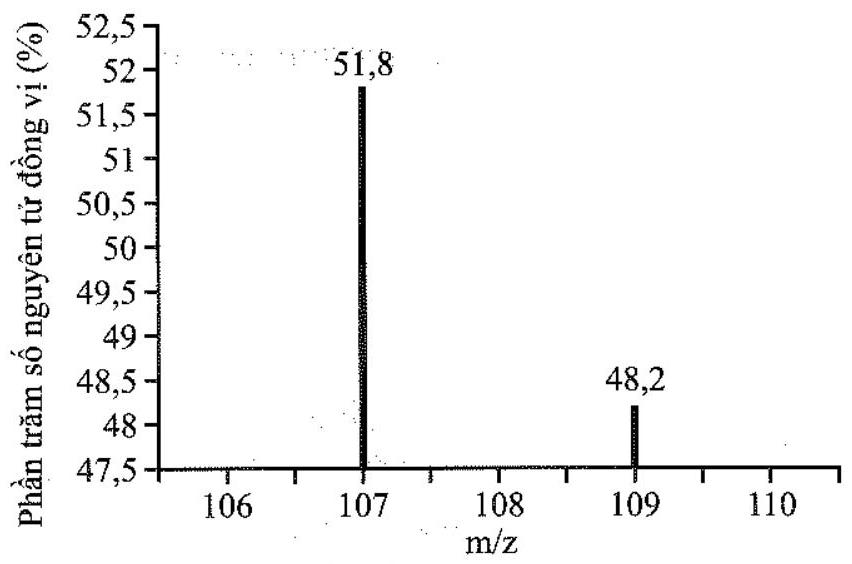
\includegraphics[max width=\textwidth, center]{2025_10_23_baf6b6057fd5ebd09626g-03}

Phổ khối lượng của bạc\\
Nguyên tử khối trung bình của Ag là 107,96 .\\
3.11. A.\\
3.12. Phản ứng (2) có xảy ra bởi vì phản ứng (1) xảy ra, vai trò của D và T là như nhau.

\section*{BAT 4}
4.1.C.\\
4.2. A. Khi nguyên tử hấp thụ năng lượng, electron sẽ chuyển từ lớp có năng lượng thấp hơn lên lớp có năng lượng cao hon.\\
4.3. A.\\
4.4. B. Số lượng electron trên một lớp tối đa là $2 n^{2}$. Lớp thứ nhất chưa tối đa 2 electron, còn 7 electron sẽ được điền vào lớp thứ hai (do lớp thứ hai có thể chưa tối đa 8 electron).\\
4.5. (1) hạt nhân; (2) quỹ đạo; (3) cao; (4) ra xa.\\
4.6. A.\\
4.7. B.\\
4.8. C.\\
4.9. (1) Đúng; (2) Sai; (3) Sai; (4) Sai.\\
4.10. A, C.\\
4.11. B. Mỗi AO chỉ chứa tối đa 2 electron.\\
4.12. Mỗi orbital nguyên tử chưa tối đa 2 electron, nên 9 electron sẽ xếp vào 5 orbital, trong đó có 4 orbital chưa 2 electron và 1 orbital chứa 1 electron. Như vậy, có 4 cặp electron ghép đôi và 1 electron độc thân.\\
4.13. Mỗi orbital nguyên tử chứa tối đa hai electron nên số lượng orbital tối thiểu tương ứng là 1,4 và 9 .\\
4.14. $0,529 \AA$ và $2,116 \AA$. Quỹ đạo thứ nhất ứng với $\mathrm{n}=1$, quỹ đạo thứ hai ứng với $\mathrm{n}=2$.\\
4.15. Bán kính quỹ đạo thứ nhất ứng với $\mathrm{n}=1$. Thay các giá trị $\mathrm{Z}=2,3,4$ cho các ion $\mathrm{He}^{+}, \mathrm{Li}^{2+}, \mathrm{Be}^{3+}$ vào biếu thức thu được $\mathrm{r}_{1}$ của $\mathrm{He}^{+}, \mathrm{Li}^{2+}, \mathrm{Be}^{3+}$ lần lượt là: $0,132 \AA ; 0,059 \AA ; 0,033 \AA$. Như vậy, khi điện tích hạt nhân tăng, bán kính quỹ đạo giảm dần (xét cùng một lớp). Điều này được giải thích là khi Z tăng, lực hút giữa hạt nhân với electron cũng sẽ tăng nên electron chuyển động về gần hạt nhân hơn.\\
4.16. Ở lớp thứ nhất, $\mathrm{n}=1$, thay các giá trị Z của $\mathrm{H}, \mathrm{He}^{+}$và $\mathrm{Li}^{2+}$ lần lượt là 1,2 và 3 vào công thức thu được $\mathrm{E}_{1}$ của $\mathrm{H}, \mathrm{He}^{+}$và $\mathrm{Li}^{2+}$ lần lượt là $-2,18 \times 10^{-18} \mathrm{~J}$; $-8,72 \times 10^{-18} \mathrm{~J}$ và $-1,96 \times 10^{-17} \mathrm{~J}$. Theo chiều tăng của điện tích hạt nhân, năng lượng của electron trở nên âm hơn. Điều này được giải thích là khi Z tăng, lực hút giữa hạt nhân với electron cũng sẽ tăng lên.

\section*{BÀI 5}
5.1. B. 5.2. A.\\
5.3. (1) Đúng; (2) Sai; (3) Sai; (4) Sai; (5) Đúng; (6) Đúng.\\
5.4. a) (1) lớp; (2) phân lớp; (3) gần bằng nhau; (4) bằng nhau; (5) lớp ngoài cùng.\\
b) (1) ba; (2) hai.\\
5.5. C.\\
5.6. $\mathrm{a}-3, \mathrm{~b}-2, \mathrm{c}-1$.\\
5.7. B.\\
5.8. B. Cation $\mathrm{Na}^{+}$có it hơn nguyên tử Na 1 electron, anion $\mathrm{F}^{-}$có nhiều hơn nguyên tử F 1 electron nên cả $\mathrm{Ne}, \mathrm{Na}^{+}$và $\mathrm{F}^{-}$đều có 10 electron.\\
5.9. $\mathrm{a}-2, \mathrm{~b}-1, \mathrm{c}-4, \mathrm{~d}-3$. Với anion $\mathrm{N}^{3-}$, số electron phải bằng số electron nguyên tử trung hoà cộng với 3 , tức là $\mathrm{N}^{3-}$ phải có 10 electron. Với cation $\mathrm{C}^{2+}$, số electron của $\mathrm{C}^{2+}$ là 4 electron.\\
5.10. A. N có 3 electron độc thân. Để xác định số electron độc thân thì cần viết cấu hình electron và biểu diễn dưới dạng ô orbital.\\
5.11. $\mathrm{a}-3, \mathrm{~b}-2, \mathrm{c}-1, \mathrm{~d}-2$. Xác định số electron lớp ngoài cùng của nguyên tử, từ đó xác định tính chất hoá học đặc trưng.\\
5.12. B. Electron hoá trị là electron lớp ngoài cùng chứ không phải phân lớp ngoài cùng. Trong trường hợp này, số electron hoá trị là 5 .\\
5.13. C. Nguyên tử nguyên tố: (2), (3), (4).\\
5.14. a) Nguyên tử O có $\mathrm{Z}=8$, cấu hình electron là $[\mathrm{He}] 2 \mathrm{~s}^{2} 2 \mathrm{p}^{4}$. Để tạo ra được $\mathrm{O}^{2-}, \mathrm{O}$ phải nhận thêm 2 electron vào orbital 2 p . Cấu hình của $\mathrm{O}^{2-}$ là $[\mathrm{He}] 2 \mathrm{~s}^{2} 2 \mathrm{p}^{6}$.\\
Để xác định số electron độc thân, cần biểu diễn dưới dạng ô orbital:

\begin{center}
\begin{tabular}{lll|l|l|l|}
O: & $[\mathrm{He}]$ & $\uparrow \downarrow$ & $\uparrow \downarrow$ & $\uparrow$ & $\uparrow$ \\
$\mathrm{O}^{2-}:$ & $[\mathrm{He}]$ & $\uparrow \downarrow$ & $\uparrow \downarrow$ & $\uparrow \downarrow$ & $\uparrow \downarrow$ \\
\cline { 2 - 5 }
 &  &  &  &  &  \\
\cline { 2 - 5 }
\end{tabular}
\end{center}

Vậy O có 2 electron độc thân, còn $\mathrm{O}^{2-}$ không có electron độc thân.\\
b) Nguyên tử Al có $\mathrm{Z}=13$, cấu hình electron là $[\mathrm{Ne}] 3 \mathrm{~s}^{2} 3 \mathrm{p}^{1}$.

Để tạo ra được $\mathrm{Al}^{3+}, \mathrm{Al}$ phải mất đi 3 electron từ orbital $3 \mathrm{p}, 3 \mathrm{~s}$. Cấu hình của $\mathrm{Al}^{3+}$ là $[\mathrm{Ne}]$ hay $[\mathrm{He}] 2 \mathrm{~s}^{2} 2 \mathrm{p}^{6}$.\\
Làm tương tự, Al có 1 electron độc thân, $\mathrm{Al}^{3+}$ không có electron độc thân.\\
5.15. Số lượng electron trong cấu hình trên là 10 .

\begin{itemize}
  \item Nếu đó là nguyên tử thì nguyên tử phải có 10 electron, do đó $Z=10$, đó là $N e$.
  \item Nếu đó là cation $\mathrm{M}^{\mathrm{n}+}(\mathrm{n}=1,2)$ thì cation này được tạo ra từ nguyên tử M bằng cách tách đi n electron. Có thể biểu diễn bằng sơ đồ: $\mathrm{M} \rightarrow \mathrm{M}^{\mathrm{n}+}$ (10 electron) + ne.\\
Vậy số electron trong nguyên tử M là: $10+\mathrm{n}$. Nếu $\mathrm{n}=1, \mathrm{M}$ có 11 electron nên $\mathrm{Z}=11$, đó là ion $\mathrm{Na}^{+}$. Nếu $\mathrm{n}=2, \mathrm{M}$ có 12 electron nên $\mathrm{Z}=12$, đây là ion $\mathrm{Mg}^{2+}$. Tương tự, với anion $\mathrm{X}^{\mathrm{n}-}: \mathrm{X}+$ ne $\rightarrow \mathrm{X}^{\mathrm{n}-}$ ( 10 electron).\\
Vậy số electron trong nguyên tử $X$ là: $10-n$. Nếu $n=1, X$ có 9 electron và $Z=9$, đây là ion $F^{-}$. Nếu $n=2, X$ có 8 electron nên $Z=8$, đây là $O^{2-}$.\\
5.16. Co có $Z=27$ nên có cấu hình electron là: $1 s^{2} 2 s^{2} 2 p^{6} 3 s^{2} 3 p^{6} 3 d^{7} 4 s^{2}$. Khi Co mất đi 2 electron và 3 electron sẽ lần lượt tạo ra $\mathrm{Co}^{2+}$ và $\mathrm{Co}^{3+}$. Các electron sẽ tách đi từ các lớp ngoài rồi tới lớp trong. Cấu hình của hai ion này là:\\
$\mathrm{Co}^{2+}: 1 \mathrm{~s}^{2} 2 \mathrm{~s}^{2} 2 \mathrm{p}^{6} 3 \mathrm{~s}^{2} 3 \mathrm{p}^{6} 3 \mathrm{~d}^{7}$;
\end{itemize}

$$
\mathrm{Co}^{3+}: 1 s^{2} 2 s^{2} 2 p^{6} 3 s^{2} 3 p^{6} 3 d^{6}
$$

Sơ đồ phân bố electron vào các ô orbital:\\
$\mathrm{Co}^{2+}:[\mathrm{Ar}]$\\
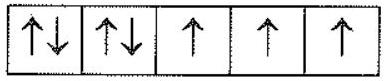
\includegraphics[max width=\textwidth, center]{2025_10_23_baf6b6057fd5ebd09626g-06}\\
$\mathrm{Co}^{3+}$ : [Ar]

\begin{center}
\begin{tabular}{|l|l|l|l|l|}
\hline
$\uparrow \downarrow$ & $\uparrow$ & $\uparrow$ & $\uparrow$ & $\uparrow$ \\
\hline
\end{tabular}
\end{center}

Số electron độc thân trong $\mathrm{Co}^{2+}$ và $\mathrm{Co}^{3+}$ lần lượt là 3 và 4 .\\
5.17. Viết cấu hình electron của bromine ( $Z=35$ ) và krypton ( $Z=36$ ), từ đó xác định số electron lớp vỏ ngoài cùng của chúng lần lượt là 7 và 8 . Do đó, bromine là phi kim điển hình, còn krypton là khí hiếm.\\
5.18. Cấu hình electron của $\mathrm{Cu}(\mathrm{Z}=29): 1 \mathrm{~s}^{2} 2 \mathrm{~s}^{2} 2 \mathrm{p}^{6} 3 \mathrm{~s}^{2} 3 \mathrm{p}^{6} 3 \mathrm{~d}^{10} 4 \mathrm{~s}^{1}$ hay $[\mathrm{Ar}] 3 \mathrm{~d}^{10} 4 \mathrm{~s}^{1}$. Cấu hình electron của $\mathrm{Cu}^{+}: 1 \mathrm{~s}^{2} 2 \mathrm{~s}^{2} 2 \mathrm{p}^{6} 3 \mathrm{~s}^{2} 3 \mathrm{p}^{6} 3 \mathrm{~d}^{10}$ hay $[\mathrm{Ar}] 3 \mathrm{~d}^{10}$.\\
Biểu diễn các cấu hình electron dưới dạng ô orbital sẽ thấy Cu có 1 electron độc thân, trong khi $\mathrm{Cu}^{+}$không có electron độc thân. Vậy Cu thuận từ còn $\mathrm{Cu}^{+}$ nghịch từ.

\section*{BAI 6}
6.1. a) B; b) C.\\
6.2. A.\\
6.3. (1): Sai. Với trường hợp nhóm B , chẳng hạn nhóm VIIIB, số thứ tự của nhóm không bằng số electron ở lớp vỏ ngoài cùng.\\
(2): Sai. Ví dụ Fe thuộc nhóm VIIIB chỉ có 2 electron ở lớp vỏ ngoài cùng. (3), (4): Đúng.\\
6.4. A.\\
6.5. C. Oxygen có 8 electron nên ở ô số 8 ; có 2 lớp electron nên ở chu kì 2 ; có 6 electron lớp ngoài cùng (trên 2 s và 2 p ) nên ở nhóm VI và là nguyên tố p nên ở nhóm A .\\
6.6. D. Sắt có 26 electron nên ở ô số 26 ; có 4 lớp electron nên ở chu kì 4 ; có 2 electron lớp ngoài cùng (trên $4 s$ ) và 6 electron ở phân lớp 3 d sát lớp ngoài cùng nên ở nhóm VIII và là nguyên tố d nên ở nhóm B.\\
6.7. A, B, E.

Fluorine ( F ) và chlorine ( Cl ) có cùng số electron lớp ngoài cùng ( 7 electron trên các phân lớp s và p ở ngoài) nên nằm cùng một nhóm. Cl có 3 lớp electron nên ở chu kì 3 , lớn hơn $F$ ở chu kì 2 (chỉ có 2 lớp electron).\\
6.8. $a-3, b-4, c-1, d-2$.\\
6.9. B.\\
$\mathrm{Na}:[\mathrm{Ne}] 3 \mathrm{~s}^{1}$ là nguyên tố khối s.\\
Cr: $[\mathrm{Ar}] 3 \mathrm{~d}^{5} 4 \mathrm{~s}^{1}$ là nguyên tố khối d (vì electron đang điền vào phân lớp 3d), chứ không phải khối s , mặc dù lớp ngoài cùng là 4 s .\\
$\mathrm{Br}:[\mathrm{Ar}] 3 \mathrm{~d}^{10} 4 \mathrm{~s}^{2} 4 \mathrm{p}^{5}$ là nguyên tố khối p vì phân lớp 3 d bên trong đã điền đầy và electron đang điền vào phân lớp 4 p .\\
$\mathrm{F}: 1 \mathrm{~s}^{2} 2 \mathrm{~s}^{2} 2 \mathrm{p}^{5}$ là nguyên tố khối p .\\
$\mathrm{Cu}:[\mathrm{Ar}] 3 \mathrm{~d}^{10} 4 \mathrm{~s}^{1}$ là nguyên tố khối d . Đây là trường hợp có cấu hình electron ngoại lệ. Với $Z=29$, cấu hình electron của Cu điền theo các quy tắc là $[\mathrm{Ar}] 3 \mathrm{~d}^{9} 4 \mathrm{~s}^{2}$ và Cu là nguyên tố khối d . Tuy nhiên, do phân lớp 3 d chỉ còn thiếu 1 electron là đạt cấu hình bão hoà, nên 1 electron từ phân lớp 4 s sẽ chuyển vào 3 d tạo thành cấu hình electron là $[\mathrm{Ar}] 3 \mathrm{~d}^{10} 4 \mathrm{~s}^{1}$.\\
6.10. D.\\
6.11. Khối s là các nguyên tố có cấu hình electron lớp ngoài cùng là $n s^{1 \div 2}$, tức là cấu hình electron đang hoàn thành phân lớp s . Phân lớp s chỉ chứa tối đa 2 electron, nên khối s chỉ có 2 cột, ứng với hai cấu hình electron lớp ngoài cùng là $n s^{1}$ và $n s^{2}$. Tương tự, khối $p$ là các nguyên tố mà cấu hình electron lớp ngoài cùng là $n s^{2} n p^{1+6}$, tức là cấu hình electron đang hoàn thành phân lớp $p$. Phân lớp p chứa được tối đa 6 electron nên khối p có 6 cột, ứng với 6 cấu hình electron lớp ngoài cùng là $n s^{2} n p^{1} \div n s^{2} n p^{6}$.\\
6.12. Vì chu kì là tập hợp các nguyên tố có cùng số lớp electron nên số lượng các ô trong một chu kì bằng số lượng electron trong một lớp. Ở lớp thứ nhất chỉ chứa tối đa 2 electron (vào phân lớp 1s); ở lớp thứ hai chứa tối đa 8 electron (vào phân lớp $2 \mathrm{~s}, 2 \mathrm{p}$ ) nên chu kì 1 có 2 nguyên tố và chu kì 2 có 8 nguyên tố. Với chu kì 3 , sau khi điền đầy phân lớp 3 s và 3 p (8 electron, ứng với số lượng 8 nguyên tố), thì chuyển sang điền electron vào phân lớp 4 s chứ không phải 3d, nên chu kì 3 chỉ có 8 nguyên tố. Chu kì 4 sẽ hoàn thiện các phân lớp 4 s , 4 p (tổng electron tối đa trên phân lớp này là 8 electron) và cả phân lớp 3 d (tối đa 10 electron) nên chu kì 4 có 18 nguyên tố.\\
6.13. Từ số hiệu nguyên tử, viết được cấu hình electron của Ca là $1 s^{2} 2 s^{2} 2 p^{6} 3 s^{2} 3 p^{6} 4 s^{2}$. Nguyên tố này ở ô thứ 20 , chu kì 4 và ở nhóm IIA.\\
6.14. Dựa vào bảng tuần hoàn có thể xác định được số thứ tự của chu kì của nguyên tố đó, cũng tức là số lớp electron, chỉ có thể nằm trong khoảng từ 1 đến 7. Kết quả thu được như sau:

\begin{center}
\begin{tabular}{|l|l|l|l|l|}
\hline
Số trong dây số & Số lóp electron (số thứ tur chu ki) & Số hiệu nguyên tữ & Ki hiệu nguyên tố & Kí hiêu mật mâ \\
\hline
8 & 2 & 6 & C & C \\
\hline
2 & 1 & 1 & H & H \\
\hline
69 & 6 & 63 & Eu & E \\
\hline
29 & 4 & 25 & Mn & M \\
\hline
58 & 5 & 53 & I & I \\
\hline
19 & 3 & 16 & S & S \\
\hline
26 & 4 & 22 & Ti & T \\
\hline
\end{tabular}
\end{center}

\begin{center}
\begin{tabular}{|c|c|c|c|c|}
\hline
\begin{tabular}{c}
Số trong \\
dãy số \\
\end{tabular} & \begin{tabular}{c}
Số lớp electron \\
(số thứ tự chu ki) \\
\end{tabular} & \begin{tabular}{c}
Số hiệu \\
nguyên từ \\
\end{tabular} & \begin{tabular}{c}
Kí hiệu \\
nguyên tố \\
\end{tabular} & \begin{tabular}{c}
Kí hiệu \\
mật mã \\
\end{tabular} \\
\hline
42 & 5 & 37 & Rb & R \\
\hline
76 & 6 & 70 & Yb & Y \\
\hline
\end{tabular}
\end{center}

Mật mã: CHEMISTRY.

\section*{BÀI 7}
7.1. a) In ; b) $\mathrm{Si} ; \mathrm{c}) \mathrm{Pb} ; \mathrm{d}) \mathrm{C}$.

Dựa vào bảng tuần hoàn, tìm vị trí các nguyên tố và áp dụng quy luật về xu hướng biến đổi bán kính nguyên tử.\\
7.2. A.\\
7.3. D. Các ion này đều có cấu hình electron là $1 s^{2} 2 s^{2} 2 p^{6} 3 s^{2} 3 p^{6}$, bán kính ion sẽ phụ thuộc vào điện tích hạt nhân. Điện tích hạt nhân càng lớn càng hút mạnh electron ở lớp ngoài cùng, bán kính sẽ càng nhỏ. Điện tích hạt nhân của $\mathrm{Ca}^{2+}, \mathrm{K}^{+}, \mathrm{Cl}^{-}, \mathrm{S}^{2-}$ lần lượt là $+20,+19,+17,+16$ nên bán kính sẽ tăng dần từ $\mathrm{Ca}^{2+}$ tới $\mathrm{S}^{2-}$.\\
7.4. B. Các cation luôn có bán kính nhỏ hơn đáng kể so với nguyên tử trung hoà tương ứng do có số lượng electron it hơn, lực hút của hạt nhân lên các electron mạnh hơn, do vậy bán kính của $\mathrm{K}^{+}$phải nhỏ hơn của $\mathrm{K}(227 \mathrm{pm})$. Bên cạnh đó, theo xu hướng biến đổi tuần hoàn thì bán kính của $\mathrm{K}^{+}$phải lớn hơn của $\mathrm{Na}^{+}(98 \mathrm{pm})$, tương tự như bán kính của K lớn hơn của Na . Trong hai giá trị 133 và 195 pm , giá trị 133 pm phù hợp hơn vì thể hiện sự giảm đáng kể bán kính cation so với nguyên tử trung hoà, tương tự như trường hợp Na và $\mathrm{Na}^{+}$ trong bảng số liệu.\\
7.5. B.\\
7.6. a) Sr ; b) Bi ; c) B ; d) As .\\
7.7. C.\\
7.8. B.\\
7.9. A. Từ cấu hình electron, xác định được nguyên tố hoá học và vị trí của chúng trong bảng tuần hoàn. Sau đó, áp dụng quy luật về xu hướng biến đổi độ âm điện.\\
7.10. (1) Li; (2) lớn nhất; (3) F; (4) nhỏ nhất; (5) Li; (6) F.\\
7.11. C . Vì độ âm điện của $\mathrm{F}>\mathrm{Cl}>\mathrm{Br}$ (các nguyên tố trong cùng một nhóm VIIA).\\
7.12. Basic oxide: $\mathrm{Na}_{2} \mathrm{O}, \mathrm{MgO}$. Acidic oxide: $\mathrm{P}_{2} \mathrm{O}_{5}, \mathrm{SO}_{3}, \mathrm{Cl}_{2} \mathrm{O}_{7}$. Oxide lưỡng tính: $\mathrm{Al}_{2} \mathrm{O}_{3}$.\\
7.13. A, B.\\
7.14. $a-4 ; b-1 ; c-2 ; d-3$.\\
7.15. Nhôm - Al thuộc nhóm IIIA, vậy eka-nhôm (Ea) thuộc nhóm IIIA cũng sẽ có 3 electron lớp ngoài cùng, công thức oxide cao nhất sẽ là $\mathrm{Ea}_{2} \mathrm{O}_{3}$, công thức hydroxide là $\mathrm{Ea}(\mathrm{OH})_{3} . \mathrm{Al}(\mathrm{OH})_{3}$ là một chất lưỡng tính nên $\mathrm{Ea}(\mathrm{OH})_{3}$ cũng có khả năng là một chất lưỡng tính, nhưng sẽ thể hiện tính base mạnh hơn $\mathrm{Al}(\mathrm{OH})_{3}$.\\
7.16. a) Lệch về phía X . b) X có bán kính nhỏ hơn do độ âm điện của X lớn hơn Y nên X sẽ nằm về bên phải Y , bán kính nguyên tử trong một chu kì giảm theo chiều từ trái sang phải. c) Oxide của X sẽ có tính acid mạnh hơn của Y .\\
7.17. M là nguyên tố kim loại nhóm IA do phản ứng với nước tạo MOH nên sẽ có 1 electron lớp ngoài cùng. Nếu M ở chu kì $4, \mathrm{M}$ sẽ có 4 lớp electron. Cấu hình electron của $M$ là $1 s^{2} 2 s^{2} 2 p^{6} 3 s^{2} 3 p^{6} 4 s^{1}$.

\section*{BÀI 8}
8.1. A.\\
8.2. B.\\
8.3. B.\\
8.4. C.\\
8.5. $\mathrm{A}, \mathrm{D}, \mathrm{G}$. Vì X và Y tạo thành hai oxide cao nhất có công thức tương tự nhau mà $\mathrm{X}, \mathrm{Y}$ là nguyên tố nhóm A , do đó chúng phải thuộc cùng một nhóm. Khi tan trong nước, các oxide này tạo dung dịch làm quỳ tím chuyển sang màu đỏ, vậy $X, Y$ là phi kim. Nguyên tử khối của $X$ nhỏ hơn của $Y$, vậy số hiệu nguyên tử của X nhỏ hơn của Y .\\
8.6. A.\\
8.7. $\mathrm{K}^{+}$có điện tích $1+$ nên cần tìm những ion có điện tích $1+$ tương tự.

Nếu xem xét $\mathrm{Ar}^{+}$và $\mathrm{Ca}^{+}$thì đây những ion có cùng điện tích và kích thước, khối lượng khá gần với $\mathrm{K}^{+}$, nhưng Ar là khí hiếm nên khó nhường 1 electron\\
tạo $\mathrm{Ar}^{+}$, còn Ca ở nhóm IIA nên tính chất hợp chất của nó sẽ khác biệt với hợp chất của K .\\
Nếu xét trong cùng một nhóm IA, có thể có $\mathrm{Na}^{+}$và $\mathrm{Rb}^{+}$sẽ có cùng số electron hoá trị và tính chất tương tự như $\mathrm{K}^{+}$nhưng bán kính của $\mathrm{Na}^{+}$sẽ nhỏ hơn, còn bán kính của $\mathrm{Rb}^{+}$lại lớn hơn nhiều so với $\mathrm{K}^{+}$.\\
8.8. C có cấu hình electron lớp vỏ ngoài cùng là $2 \mathrm{~s}^{2} 2 \mathrm{p}^{2}$, thuộc nhóm IVA. Nguyên tố cùng nhóm IVA khác có thể có những tính chất tương tự C nhất là Si .\\
8.9. a) Có thể xây dựng đồ thị phụ thuộc khối lượng riêng vào bán kính nguyên tử, sau đó dựa vào đồ thị để tìm ra khối lượng riêng của Kr khoảng 3,40 .\\
Trong trường hợp gần đúng đơn giản hơn, có thể suy luận trong khoảng khối lượng riêng của Ar và Xe . Kết quả ra khoảng 3,65 . Cụ thể: Khi tăng bán kính từ 71 lên 108 thì khối lượng riêng tăng từ 1,78 lên 5,85 . Vậy khi bán kính nguyên tử tăng lên 1 đơn vị, khối lượng riêng tăng thêm một lượng là:

$$
\frac{5,85-1,78}{108-71}=0,11
$$

Khối lượng riêng của Kr có thể tính từ khối lượng riêng của Ar là:

$$
1,78+(88-71) \times 0,11=3,65\left(\mathrm{~g} \mathrm{~L}^{-1}\right)
$$

Kết quả thực nghiệm, khối lượng riêng của Kr là $3,70 \mathrm{~g} \mathrm{~L}^{-1}$. Như vậy, kết quả ước tính khá gần với kết quả thực nghiệm.\\
b) Khối lượng của một nguyên tử Ne là:

$$
\frac{20,18}{6,02 \times 10^{23}}=3,35 \times 10^{-23}(\mathrm{~g})
$$

Thể tích của một nguyên tử Ne là:

$$
\frac{4}{3} \pi \mathrm{r}^{3}=\frac{4}{3} \times 3,14 \times\left(38 \times 10^{-12}\right)^{3}=2,30 \times 10^{-31}\left(\mathrm{~m}^{3}\right)=2,30 \times 10^{-28}(\mathrm{~L})
$$

Khối lượng riêng của nguyên tử Ne là:

$$
\frac{3,35 \times 10^{-23}}{2,30 \times 10^{-28}}=1,46 \times 10^{5}\left(\mathrm{~g} \mathrm{~L}^{-1}\right)
$$

Khối lượng riêng của nguyên tử Ne lớn hơn rất nhiều so với khối lượng riêng của khí Ne. Điều đó cho thấy, trong khí neon, các nguyên tử phải ở rất xa nhau.\\
8.10. $X$ thuộc chu kì 8 , nhóm IA, là kim loại điển hình. Y thuộc chu kì 8 , nhóm IIA, là kìm loại điển hình.

\section*{BÀI 9}
9.1. B. Oxygen là phi kim, có xu hướng nhận electron. Cấu hình electron của oxygen có lớp vỏ ngoài cùng là $2 \mathrm{~s}^{2} 2 \mathrm{p}^{4}$, còn thiếu 2 electron nữa thì đạt được cấu hình lớp vỏ thoả măn quy tắc octet.\\
9.2. A. Sodium (Na) là một kim loại điển hình nên có xu hướng nhường electron. Cấu hình electron của Na có lớp vỏ ngoài cùng là $3 \mathrm{~s}^{1}$, nhường đi 1 electron thì đạt cấu hình của khí hiếm Ne ứng với lớp vỏ thoả mãn quy tắc octet.\\
9.3. A. Silicon nằm ở nhóm IVA trong bảng tuần hoàn nên khi nhường hoặc nhận 4 electron sẽ tạo thành cấu hình bền vững của khí hiếm. Nó còn được gọi là á kim.\\
9.4. D. Hydrogen không thể đạt được lớp vỏ thoả mãn quy tắc octet mà chỉ có thể đạt được lớp vỏ của khí hiếm gần nó nhất là helium (2 electron).\\
9.5. D. Chlorine là phi kim có xu hướng nhận electron.\\
9.6. $\mathrm{a}-2, \mathrm{~b}-1, \mathrm{c}-3, \mathrm{~d}-4$.\\
9.7. C. Nguyên tử này có 15 electron và nhận thêm 3 electron để đạt được lớp vỏ thoả mãn quy tắc octet, vậy đó là phosphorus.\\
9.8. B. Nguyên tử này có 19 electron, có 1 electron lớp vỏ ngoài cùng nên dễ nhường 1 electron để đạt được cấu hình của khí hiếm với lớp vỏ thoả mãn quy tắc octet.\\
9.9. A. Nguyên tử có 13 electron, có 3 electron lớp vỏ ngoài cùng, nên là một kim loại, có xu hướng nhường đi 3 electron lớp vỏ ngoài cùng đó để đạt được lớp vỏ thoả mãn quy tắc octet. Vậy điện tích của ion đó là $3+$.\\
9.10.\\
a)\\
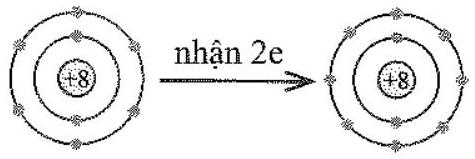
\includegraphics[max width=\textwidth, center]{2025_10_23_baf6b6057fd5ebd09626g-12(1)}\\
b)\\
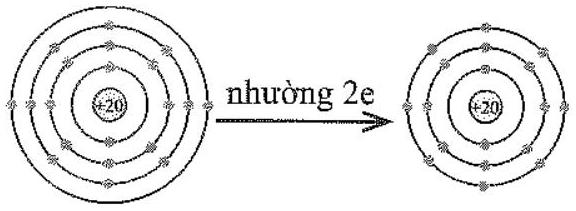
\includegraphics[max width=\textwidth, center]{2025_10_23_baf6b6057fd5ebd09626g-12(2)}\\
c)\\
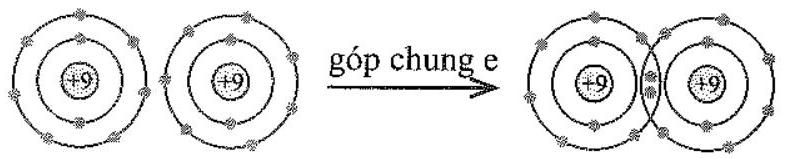
\includegraphics[max width=\textwidth, center]{2025_10_23_baf6b6057fd5ebd09626g-12}

\section*{BÀI 10}
10.1.

\begin{center}
\begin{tabular}{|l|ll|l|}
\hline
\multicolumn{1}{c}{\begin{tabular}{c}
Hợ chất tạo nêm \\
bỏi các ion đơn nguyên tử \\
\end{tabular}} & \multicolumn{2}{|c|}{\begin{tabular}{c}
Họp chất tạ nên bỏi ion \\
đơn nguyên tữ và đa nguyên tưr \\
\end{tabular}} & \begin{tabular}{c}
Hơp chất tạo nên bởi \\
các ion đa nguyên tữ \\
\end{tabular} \\
\hline
$\mathrm{KCl}, \mathrm{AgCl}$ & \begin{tabular}{l}
$\mathrm{Na}_{2} \mathrm{CO}_{3}, \mathrm{BaCO}_{3}, \mathrm{BaSO}_{4}$, \\
$\mathrm{KMnO}_{4}$ \\
\end{tabular} & $\left(\mathrm{NH}_{4}\right)_{2} \mathrm{SO}_{4}$ &  \\
\hline
\end{tabular}
\end{center}

10.2. C.\\
10.3. D. Liên kết ion được tạo thành giữa kim loại và phi kim.\\
10.4. A, D, E, H.\\
10.5. C. Bán kính của O nhỏ hơn của $\mathrm{O}^{2-}$ do khi nhận thêm electron thì lực đẩy giữa các electron sẽ tăng lên, làm giảm lực hút giữa hạt nhân với các electron, dẫn đến electron ở xa hạt nhân hơn.\\
10.6. B. Bán kính của Al lớn hơn của $\mathrm{Al}^{3+}$ do khi hình thành cation, nguyên tử mất bớt electron, lực hút của hạt nhân với các electron tăng lên, electron sẽ ở gần hạt nhân hơn.\\
10.7. $a-3, b-2, c-4, d-1$.\\
10.8. E.\\
10.9. (1) ion; (2) rắn; (3) $\mathrm{Ba}^{2+}$; (4) $\mathrm{I}^{-}$.\\
10.10. Giai đoạn 1: Hình thành ion trái dấu theo quy tắc octet từ các quá trình kim loại $(\mathrm{Ca})$ nhường electron và phi kim $(\mathrm{F})$ nhận electron.

\begin{center}
\begin{tabular}{lcll}
 & Ca & $\rightarrow$ & $\mathrm{Ca}^{2+}+2 \mathrm{e}$ \\
Cấu hình electron & $[\mathrm{Ar}] 4 \mathrm{~s}^{2}$ &  & $[\mathrm{Ar}]$ \\
 & $\mathrm{F}+1 \mathrm{e}$ & $\rightarrow$ & $\mathrm{F}^{-}$ \\
Cấu hình electron & $[\mathrm{He}] 2 \mathrm{~s}^{2} 2 \mathrm{p}^{5}$ & $[\mathrm{Ne}]$ &  \\
\end{tabular}
\end{center}

Giai đoạn 2: Các ion trái dấu hút nhau bằng lực hút tĩnh điện tạo nên hợp chất ion.

$$
\mathrm{Ca}^{2+}+2 \mathrm{~F}^{-} \rightarrow \mathrm{CaF}_{2}
$$

10.11. Sau khi được hình thành, các cation và anion sẽ hút nhau bởi lực đĩnh điện rất mạnh để tạo thành hợp chất ion, quá trình này giải phóng nhiều năng lượng (thậm chí dư thừa để bù cho các quá trình đã hấp thu năng lượng trước đó, chẳng hạn năng lượng để phá vỡ liên kết $\mathrm{Cl}-\mathrm{Cl}$ ).\\
10.12. a) LiCl : do khi tạo thành hợp chất LiCl hay NaCl thì đều đi từ các cation có điện tích $1+$ và anion có điện tích $1-$, nhưng bán kính của $\mathrm{Li}^{+}$nhỏ hơn của $\mathrm{Na}^{+}$nên lực hút tĩnh điện giữa $\mathrm{Li}^{+}$với $\mathrm{Cl}^{-}$sẽ mạnh hơn và toả ra nhiều năng lượng hơn so với $\mathrm{Na}^{+}$.\\
b) MgO : do khi tạo thành $\mathrm{Na}_{2} \mathrm{O}$ thì cation mang điện tích $1+\left(\mathrm{Na}^{+}\right)$, còn khi tạo thành MgO thì cation mang điện tích $2+\left(\mathrm{Mg}^{2+}\right)$ nên lực hút giữa $\mathrm{Mg}^{2+}$ với $\mathrm{O}^{2-}$ sẽ mạnh hơn nhiều so với giữa $\mathrm{Na}^{+}$và $\mathrm{O}^{2-}$, do đó năng lượng toả ra khi tạo thành MgO cũng nhiều hơn.

\section*{BÀI 11}
11.1. C. Trong nguyên tử C , electron có khả năng tham gia hình thành liên kết cộng hoá trị là những electron thuộc lớp vỏ ngoài cùng.\\
11.2. D, E.\\
11.3. B.\\
11.4. B.\\
11.5. A.\\
11.6. B . Đó là các nguyên tử B và Be .\\
11.7. B. Trường hợp (4) không đúng vì $P$ bị thiếu một cặp electron riêng.\\
11.8. A.\\
11.9. (1) hai,\\
(2) bốn,\\
(3) hai,\\
(4) CsF ,\\
(5) NaF ,\\
(6) một,\\
(7) $\mathrm{H}_{2} \mathrm{O}$,\\
(8) NaF ,\\
(9) $\mathrm{H}_{2} \mathrm{O}$,\\
(10) $\mathrm{SO}_{2}$,\\
(11) $\mathrm{Cl}_{2}$,\\
(12) $\mathrm{O}_{2}$.\\
11.10. $\mathrm{a}-3, \mathrm{~b}-2, \mathrm{c}-1$.\\
11.11. C.\\
11.12. D. Mỗi nguyên tử sử dụng 3 AO 2 p , mỗi AO chứa 1 electron độc thân để tham gia xen phủ, tạo thành 3 liên kết.\\
11.13. C.\\
11.14. A. Vẫn có thể có AO s xen phủ với AO p , ví dụ như trong HF.\\
11.15. B. Mỗi liên kết hình thành do dùng chung 1 cặp (tức là 2 ) electron.\\
11.16. $\mathrm{N}_{2}$ : (1), (3), (5); Ar: (4); CO: (2), (3), (5); $\mathrm{H}_{2}$ : (1), (6).\\
11.17. B, C, G.\\
11.18. A, C, E, H.\\
11.19. D.\\
11.20. $\mathrm{C}, \mathrm{D}$. Năng lượng liên kết càng thấp, liên kết càng kém bền và càng dễ bị phá vỡ.\\
11.21. $\mathrm{E}=\frac{436 \times 10^{3}}{\mathrm{~N}_{\mathrm{A}} \times 1,602 \times 10^{-19}}=\frac{436 \times 10^{3}}{6,02 \times 10^{23} \times 1,602 \times 10^{-19}}=4,52(\mathrm{eV})$.\\
11.22.\\
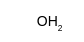
\includegraphics{smile-ea9e0150f75bc402b8a96b6d6ef480c9ab57f577}\\
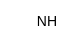
\includegraphics{smile-dd4d8f6e9ff15b828faafdcf81f0ab21a84af7b4}\\
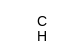
\includegraphics{smile-d33e493f93455b8fcc8672c15fd332afe978e87d}

Số cặp electron riêng của $\mathrm{H}_{2} \mathrm{O}, \mathrm{NH}_{3}$ và $\mathrm{CH}_{4}$ lần lượt là 2,1 và 0 .\\
11.23. a) Tổng năng lượng liên kết là $2 \mathrm{E}_{\mathrm{H}-\mathrm{X}}$ với X là $\mathrm{S}, \mathrm{O}$.

Năng lượng liên kết trong $\mathrm{H}_{2} \mathrm{~S}$ là: $368 \times 2=736\left(\mathrm{~kJ} \mathrm{~mol}^{-1}\right)$.\\
Năng lượng liên kết trong $\mathrm{H}_{2} \mathrm{O}$ là: $464 \times 2=928\left(\mathrm{~kJ} \mathrm{~mol}^{-1}\right)$.\\
b) Nhiệt độ bắt đầu phân huỷ của $\mathrm{H}_{2} \mathrm{O}$ cao hơn do liên kết $\mathrm{H}-\mathrm{O}$ bền hơn $\mathrm{H}-\mathrm{S}$.\\
11.24. Năng lượng liên kết $\mathrm{F}-\mathrm{F}$ là $159 \mathrm{~kJ} \mathrm{~mol}^{-1}$, liên kết $\mathrm{N} \equiv \mathrm{N}$ là $946 \mathrm{~kJ} \mathrm{~mol}^{-1}$ nên phân tử $\mathrm{F}_{2}$ sẽ dễ tham gia phản ứng với $\mathrm{H}_{2}$ hơn so với $\mathrm{N}_{2}$ do liên kết $\mathrm{F}-\mathrm{F}$ dễ bị phá vỡ hơn.\\
11.25. Bản chất liên kết ion trong NaCl là lực hút tĩnh điện giữa các ion trái dấu, không có tính định hướng. Do vậy, một ion $\mathrm{Na}^{+}$có thể hút nhiều ion $\mathrm{Cl}^{-}$xung quanh và ngược lại, dẫn tới ở điều kiện thường trong tinh thể NaCl , một ion được bao quanh bởi nhiều ion trái dấu thay vì phân tử NaCl chỉ có 2 ion.

\section*{BÀI 12}
12.1. D.\\
12.2. A. Chỉ có $\mathrm{H}_{2} \mathrm{O}, \mathrm{NH}_{3}$, HF mới tạo được liên kết hydrogen với các phân tử cùng loại, còn $\mathrm{H}_{2} \mathrm{~S}, \mathrm{CO}_{2}, \mathrm{HCl}$ thì không.\\
12.3. A.\\
12.4. C. Giữa các phân tử không phân cực hoặc giữa các nguyên tử khí hiếm vẫn có thời điểm xuất hiện sự phân cực tạm thời (do nguyên tử chứa các hạt mang điện là proton và electron), do đó luôn có tương tác van der Waals.\\
12.5. D.\\
12.6. B.\\
12.7. B.\\
12.8. A. Giữa các phân tử $\mathrm{CH}_{3} \mathrm{OH}$ có thể hình thành liên kết hydrogen.\\
12.9. D. Do $\mathrm{I}_{2}$ có khối lượng phân tử lớn nhất và đồng thời có kích thưởc lớn nhất nên tương tác van der Waals giữa các phân tử mạnh hơn.\\
12.10. Phân tử $\mathrm{CH}_{3}-\mathrm{F}$ có tương tác giữa các phân tử mạnh hơn do có liên kết $\mathrm{C}-\mathrm{F}$ phân cực hơn hơn liên kết $\mathrm{C}-\mathrm{C}$ trong phân tử $\mathrm{CH}_{3}-\mathrm{CH}_{3}$.\\
12.11. Do khối lượng nguyên tử tăng dần và theo chiều tăng của $Z$, số electron và kích thước nguyên tử tăng dần gây nên sự phân cực tạm thời của nguyên tử mạnh hơn nên tương tác van der Waals mạnh dần lên.\\
12.12.\\
12.13. Giữa các phân tử HF có liên kết hydrogen nên nhiệt độ nóng chảy cao hơn so với HCl . Từ HCl tới HI do kích thước nguyên tử halogen tăng, tương tác van der Waals giữa các phân tử tăng nên nhiệt độ nóng chảy tăng.\\
12.14. Ba chất có khối lượng phân tử tương đương nhau nên chất có nhiệt độ sôi cao nhất là chất có thể hình thành liên kết hydrogen, đó là 1-hexanol.

Chất có phân tử phân cực sẽ có liên kết van der Waals giữa các phân tử mạnh hơn, có nhiệt độ sôi xếp thứ hai (ảnh hưởng của liên kết hydrogen tới nhiệt độ sôi là mạnh hơn tương tác van der Waals), do đó chất phân cực là 2-hexanone. Còn lại là heptane.

\section*{BÀI 13}
13.1. A.\\
13.2. C . Số oxi hoá của H trong các hydride kim loại bằng -1 .\\
13.3. C.\\
13.4. A.\\
13.5. C.\\
13.6.\\
a) $\stackrel{+5}{\mathrm{~N}} \mathrm{O}_{3}^{-} ; \stackrel{+1+5-2}{\mathrm{H}_{2}} \stackrel{+}{\mathrm{PO}} \mathrm{O}_{4}^{-} ; \stackrel{+2}{\mathrm{Ca}} \stackrel{+1+5}{\mathrm{HAs}} \stackrel{-2}{\mathrm{O}}_{4} ; \stackrel{+2}{\mathrm{Mg}}_{2} \stackrel{+4-2}{\mathrm{TiO}_{4}}$.\\
b) a - 2 ; b - 5 ; c - 4 ; d - 3 ; e - 1 .\\
$+2+4-2 \quad+1 \quad+6-2 \quad-3+1 \quad+2-1$\\
13.7. $\mathrm{CaCO}_{3} ; \mathrm{H}_{2} \mathrm{SO}_{4} ; \mathrm{NH}_{4}^{+} ; \mathrm{CaH}_{2}$.\\
13.8. $\mathrm{Fe}_{3} \mathrm{O}_{4}$ được coi là hỗn hợp của hai oxide: FeO và $\mathrm{Fe}_{2} \mathrm{O}_{3}$ với số oxi hoá của nguyên tữ Fe tương ứng là: $+2,+3$.\\
13.9. A, C, E, G.\\
13.10. B, C, D.\\
13.11. (1) oxi hoá - khử; (2) số oxi hoá; (3) chất khử; (4) nhường 2; (5) chất oxi hoá; (6) nhận 3.\\
13.12. a) $4 \mathrm{FeS}_{2}+11 \mathrm{O}_{2} \xrightarrow{\mathrm{t}^{\circ}} 2 \mathrm{Fe}_{2} \mathrm{O}_{3}+8 \mathrm{SO}_{2} \uparrow$

Phản ứng (1) là phản ứng oxi hoá - khử; chất oxi hoá: $\mathrm{O}_{2}$; chất khử: $\mathrm{FeS}_{2}$.


\begin{equation*}
2 \mathrm{SO}_{2}+\mathrm{O}_{2} \xrightarrow[\mathrm{~V}_{2} \mathrm{O}_{5}]{\mathrm{t}^{\circ}} 2 \mathrm{SO}_{3} \tag{2}
\end{equation*}


Phản ứng (2) là phản ứng oxi hoá - khử; chất oxi hoá: $\mathrm{O}_{2}$; chất khử: $\mathrm{SO}_{2}$.


\begin{equation*}
\mathrm{SO}_{3}+\mathrm{H}_{2} \mathrm{O} \rightarrow \mathrm{H}_{2} \mathrm{SO}_{4} \tag{3}
\end{equation*}


Phản ứng (3) không là phản ứng oxi hoá - khử.\\
b) 1 tấn quặng chứa $60 \% \mathrm{FeS}_{2}\left(\mathrm{M}=120 \mathrm{~g} \mathrm{~mol}^{-1}\right)$.

Số mol $\mathrm{FeS}_{2}$ trong 1 tấn quặng trên là: 5000 mol .

Từ (1), (2) và (3): $5000 \mathrm{~mol} \mathrm{FeS}_{2}$ sẽ tạo được $10000 \mathrm{~mol} \mathrm{H}_{2} \mathrm{SO}_{4}$ hay 1 tấn $\mathrm{H}_{2} \mathrm{SO}_{4} 98 \%$. Tuy nhiên, hiệu suất chỉ $80 \%$ nên thực tế chỉ thu được 0,8 tấn $\mathrm{H}_{2} \mathrm{SO}_{4} 98 \%$.\\
c) $\mathrm{Fe}^{-}-\begin{gathered}\mathrm{S} \\ \mathrm{I} \\ \mathrm{S}\end{gathered}$\\
13.13. C. (1) $\mathrm{PCl}_{3}$ là chất khử, $\mathrm{Cl}_{2}$ là chất oxi hoá.

Quá trình oxi hoá: $\stackrel{+3}{\mathrm{P}} \rightarrow \stackrel{+5}{\mathrm{P}}+2 \mathrm{e}$\\
Quá trình khử: $\quad \stackrel{0}{\mathrm{Cl}}+2 \mathrm{e} \rightarrow 2 \stackrel{-1}{\mathrm{Cl}}$\\
(2) Cu là chất khử, $\mathrm{AgNO}_{3}$ là chất oxi hoá.

Quá trình oxi hoá: $\stackrel{0}{\mathrm{Cu}} \rightarrow \stackrel{+2}{\mathrm{Cu}}+2 \mathrm{e}$\\
Quá trình khử: $\quad \stackrel{+1}{\mathrm{Ag}}+\mathrm{e} \rightarrow \stackrel{0}{\mathrm{Ag}}$\\
13.14. Chất bị oxi hoá: a) $\mathrm{H}_{3} \mathrm{AsO}_{3}$; b) $\mathrm{NaI} ;$ c) $\mathrm{H}_{2} \mathrm{C}_{2} \mathrm{O}_{4}$; d) Al . Chất bị khử: a) $\mathrm{HNO}_{3}$; b) $\left.\mathrm{HOCl} ; \mathrm{c}\right) \mathrm{KMnO}_{4}$; d) $\mathrm{H}_{2} \mathrm{SO}_{4}$.\\
13.15. a) $\stackrel{0}{\mathrm{Ag}} \rightarrow \stackrel{+1}{\mathrm{Ag}}+1 \mathrm{e} ; \quad \stackrel{+2}{\mathrm{Fe}}+2 \mathrm{e} \rightarrow \stackrel{0}{\mathrm{Fe}} 2 \mathrm{Ag}+\mathrm{Fe}^{2+} \rightarrow 2 \mathrm{Ag}^{+}+\mathrm{Fe}$\\
b) $\stackrel{0}{\mathrm{Zn}} \rightarrow \stackrel{+2}{\mathrm{Zn}}+2 \mathrm{e} ; \quad \stackrel{+3}{\mathrm{Cr}}+3 \mathrm{e} \rightarrow \stackrel{0}{\mathrm{Cr}} 3 \mathrm{Zn}+2 \mathrm{Cr}^{3+} \rightarrow 3 \mathrm{Zn}^{2+}+2 \mathrm{Cr}$\\
c) $\stackrel{-4}{\mathrm{C}} \rightarrow \stackrel{+4}{\mathrm{C}}+8 \mathrm{e} ; \quad \stackrel{0}{\mathrm{O}_{2}}+4 \mathrm{e} \rightarrow 2 \mathrm{O}^{-2} \mathrm{CH}_{4}+2 \mathrm{O}_{2} \rightarrow \mathrm{CO}_{2}+2 \mathrm{H}_{2} \mathrm{O}$\\
d) $\stackrel{0}{\mathrm{Al}} \rightarrow \stackrel{+3}{\mathrm{Al}}+3 \mathrm{e} ; \quad \stackrel{+4}{\mathrm{Mn}}+4 \mathrm{e} \rightarrow \stackrel{0}{\mathrm{Mn}} 3 \mathrm{MnO}_{2}+4 \mathrm{Al} \rightarrow 3 \mathrm{Mn}+2 \mathrm{Al}_{2} \mathrm{O}_{3}$\\
13.16. $2 \mathrm{NaN}_{3} \rightarrow 2 \mathrm{Na}+3 \mathrm{~N}_{2}$

Phản ứng này là phản ứng oxi hoá - khử vì trong phản ứng có sự nhường electron và nhận electron. Số oxi hoá của Na và N trong hợp chất lần lượt là: +1 và $-\frac{1}{3}$.\\
13.17. Du oxygen: $2 \mathrm{C}_{8} \mathrm{H}_{18}+25 \mathrm{O}_{2} \rightarrow 16 \mathrm{CO}_{2}+18 \mathrm{H}_{2} \mathrm{O}$.

Không dư oxygen: $\mathrm{C}_{8} \mathrm{H}_{18}+\frac{17}{2} \mathrm{O}_{2} \rightarrow 8 \mathrm{CO}+9 \mathrm{H}_{2} \mathrm{O}$.

Rất thiếu oxygen: $\mathrm{C}_{8} \mathrm{H}_{18}+\frac{9}{2} \mathrm{O}_{2} \rightarrow 8 \mathrm{C}+9 \mathrm{H}_{2} \mathrm{O}$.\\
Điều kiện cháy dư oxygen sẽ tiết kiệm năng lượng nhất và không gây ô nhiễm môi trường. Trong điều kiện đó, một phân tử $\mathrm{C}_{8} \mathrm{H}_{18}$ nhường 50 electron.

\section*{BÀI 14}
14.1. A, B, D.

C : Ví dụ phản ứng phân huỷ nước, phản ứng nung vôi $\left(\mathrm{CaCO}_{3}\right)$ là những phản ứng thu nhiệt.\\
E : Phản ứng $\mathrm{H}_{2}(g)+\frac{1}{2} \mathrm{O}_{2}(g) \rightarrow \mathrm{H}_{2} \mathrm{O}(g)$ có $\Delta_{\mathrm{r}} \mathrm{H}_{298}^{0}=-241,8 \mathrm{~kJ}$.\\
Nhưng phản ứng $\mathrm{H}_{2}(g)+\frac{1}{2} \mathrm{O}_{2}(g) \rightarrow \mathrm{H}_{2} \mathrm{O}(l)$ có $\Delta_{\mathrm{r}} \mathrm{H}_{298}^{0}=-285,8 \mathrm{~kJ}$.\\
G: Việc đốt củi ban đầu cần phải khơi mào cho củi cháy nhưng sau đó phản ứng cháy có thể tự tiếp diễn và toả rất nhiều nhiệt.\\
14.2. B, D.\\
14.3. A.\\
14.4. (1) Thu nhiệt; (2) Toả nhiệt; (3) Thu nhiệt; (4) Toả nhiệt.\\
14.5. C. Năng lượng giải phóng khi đốt 15,1 gam ethanol là:

$$
\frac{15,1}{46} \times\left(1,37 \times 10^{3}\right)=4,50 \times 10^{2}(\mathrm{~kJ})
$$

14.6. D.\\
14.7. B, D.\\
14.8. B, C.\\
14.9. a) thu;\\
b) $-241,8 \mathrm{~kJ} \mathrm{~mol}^{-1}$;\\
c) $-483,6 \mathrm{~kJ}$;\\
d) $241,8 \mathrm{~kJ}$.\\
14.10. C.\\
14.11. Phản ứng toả nhiệt. Cần nhỏ từ từ $\mathrm{H}_{2} \mathrm{SO}_{4}$ đặc vào nước. Nếu làm ngược lại, do phản ứng toả nhiệt rất mạnh sẽ làm bắn $\mathrm{H}_{2} \mathrm{SO}_{4}$ ra xung quanh, gây mất an toàn và làm hư hại đồ vật, quần áo,...\\
14.12. Lượng nhiệt cần để đun nóng 500 gam nước từ $20^{\circ} \mathrm{C}$ lên $90^{\circ} \mathrm{C}$ là:

$$
\frac{500}{18} \times 75,4 \times(363-293)=146611,1(\mathrm{~J}) .
$$

Vậy lượng than cần dùng là: $146611,1:\left(23 \times 10^{3}\right)=6,37(\mathrm{~g})$.\\
14.13. Lượng nhiệt cần dùng là:

$$
[1,44 \times(78,29-20)+855] \times 10^{3}=9,39 \times 10^{5}(\mathrm{~J}) .
$$

\section*{BÀI 15}
15.1. $\mathrm{a}-4 ; \mathrm{b}-1 ; \mathrm{c}-3 ; \mathrm{d}-2$.\\
15.2. a) Phản ứng đó toả nhiệt vì có biến thiên enthalpy âm.\\
b) Phản ứng thuỷ phân đường sucrose trong môi trường acid và đun nóng;

$$
\mathrm{C}_{12} \mathrm{H}_{22} \mathrm{O}_{11}+\mathrm{H}_{2} \mathrm{O} \rightarrow \mathrm{C}_{6} \mathrm{H}_{12} \mathrm{O}_{6} \text { (glucose) }+\mathrm{C}_{6} \mathrm{H}_{12} \mathrm{O}_{6} \text { (fructose) }
$$

Phản ứng trong sơ đồ là phản ứng oxi hoá - khử; oxygen là chất oxi hoá, đường glucose và fructose là chất khử.

$$
\mathrm{C}_{6} \mathrm{H}_{12} \mathrm{O}_{6}(s)+6 \mathrm{O}_{2}(g) \rightarrow 6 \mathrm{CO}_{2}(g)+6 \mathrm{H}_{2} \mathrm{O}(l)
$$

c) Phản ứng đốt cháy đường sucrose:

$$
\mathrm{C}_{12} \mathrm{H}_{22} \mathrm{O}_{11}(s)+12 \mathrm{O}_{2}(g) \rightarrow 12 \mathrm{CO}_{2}(g)+11 \mathrm{H}_{2} \mathrm{O}(l)
$$

Biến thiên enthalpy chuẩn của phản ứng là: -5645 kJ .\\
d) $\frac{5}{342} \times(-5645)=-82,5(\mathrm{~kJ})$.\\
e) Cơ thể cần năng lượng để hoạt động nên phải có chế độ dinh dưỡng đầy đủ. Luyện tập thể dục, thể thao hợp lí giúp đốt cháy năng lượng dư thừa trong cơ thể.\\
15.3. a) Quá trình tan chảy của nước đá là quá trình thu nhiệt vì có biến thiên enthalpy dương.\\
b) Viên đá tan chảy dần vì nó lấy nhiệt từ nước lỏng (là môi trường xung quanh).\\
c) Nước lỏng nhường nhiệt cho viên nước đá, sự mất nhiệt làm cho nước lỏng lạnh đi.\\
d) Nhiệt lượng mà 500 gam nước lỏng từ $20^{\circ} \mathrm{C}$ giảm xuống $0^{\circ} \mathrm{C}$ toả ra là:

$$
\frac{500}{18} \times 75,4 \times|0-20|=41888,9(\mathrm{~J})=41,8889(\mathrm{~kJ}) .
$$

Phần nhiệt lượng toả ra này được viên nước đá hấp thụ để tan chảy. Số viên nước đá tối thiểu cần là 7 viên ( $41888,9: 6020=6,96$ ).\\
e) Nhiệt lượng toả ra khi nhiệt độ của 120 gam nước lỏng từ $45^{\circ} \mathrm{C}$ giảm xuống $0^{\circ} \mathrm{C}$ là:

$$
\frac{120}{18} \times 75,4 \times|0-45|=22620(\mathrm{~J})
$$

Lượng nước đá cần dùng là: ( $22620: 6020$ ) $\times 18=67,63(\mathrm{~g})$.\\
Vậy dùng 150 gam nước đá là dư.\\
15.4. a) G.\\
b) $\mathrm{C}_{2} \mathrm{H}_{5} \mathrm{OH}(l)+3 \mathrm{O}_{2}(g) \rightarrow 2 \mathrm{CO}_{2}(g)+3 \mathrm{H}_{2} \mathrm{O}(l) \quad \Delta_{\mathrm{r}} \mathrm{H}_{298}^{0}=-1367,0 \mathrm{~kJ}$

$$
\begin{aligned}
\Delta_{\mathrm{r}} \mathrm{H}_{298}^{0}=3 \times \Delta_{\mathrm{f}} \mathrm{H}_{298}^{0}\left(\mathrm{H}_{2} \mathrm{O}(l)\right)+2 \times \Delta_{\mathrm{f}} \mathrm{H}_{298}^{0}\left(\mathrm{CO}_{2}(g)\right) & -3 \times \Delta_{\mathrm{f}} \mathrm{H}_{298}^{0}\left(\mathrm{O}_{2}(g)\right) \\
& -\Delta_{\mathrm{f}} \mathrm{H}_{298}^{0}\left(\mathrm{C}_{2} \mathrm{H}_{5} \mathrm{OH}(l)\right)
\end{aligned}
$$

Vậy $\Delta_{\mathrm{f}} \mathrm{H}_{298}^{0}\left(\mathrm{C}_{2} \mathrm{H}_{5} \mathrm{OH}(l)\right)=3 \times(-285,8)+2 \times(-393,5)-3 \times 0-(-1367,0)$

$$
=-277,4\left(\mathrm{~kJ} \mathrm{~mol}^{-1}\right)
$$

15.5. B, C, D, E.\\
15.6. a) $\mathrm{Fe}_{2} \mathrm{O}_{3}(s)+3 \mathrm{CO}(g) \rightarrow 2 \mathrm{Fe}(s)+3 \mathrm{CO}_{2}(g) \Delta_{\mathrm{r}} \mathrm{H}_{298}^{0}=3 \times(-393,5)+2 \times 0-3 \times(-110,5)-(-824,2)=-24,8(\mathrm{~kJ})$.\\
b) A. Tính theo số mol của CO .\\
15.7. a) $2 \mathrm{Al}(s)+3 \mathrm{Cl}_{2}(g) \rightarrow 2 \mathrm{AlCl}_{3}(s)$; đây là phản ứng oxi hoá - khử vì có sự thay đổi số oxi hoá của các nguyên tử trong phản ứng.\\
b) $\Delta_{\mathrm{r}} \mathrm{H}_{298}^{0}=-1390,81 \mathrm{~kJ}$; phản ứng trên toả nhiệt.\\
c) $52,09 \mathrm{~kJ}$.\\
d) 0,0388 gam Al.\\
15.8. a) $\mathrm{H}_{3} \mathrm{C}-\mathrm{CH}_{2}-\mathrm{CH}_{2}-\mathrm{CH}_{3} \rightarrow \mathrm{CH}_{2}=\mathrm{CH}-\mathrm{CH}=\mathrm{CH}_{2}+2 \mathrm{H}_{2}$

$$
\begin{aligned}
\Delta_{\mathrm{r}} \mathrm{H}_{298}^{0} & =\left(10 \mathrm{E}_{\mathrm{C}-\mathrm{H}}+3 \mathrm{E}_{\mathrm{C}-\mathrm{C}}\right)-\left(6 \mathrm{E}_{(\mathrm{C}-\mathrm{H})}+2 \mathrm{E}_{\mathrm{C}=\mathrm{C}}+\mathrm{E}_{\mathrm{C}-\mathrm{C}}\right)-2 \mathrm{E}_{\mathrm{H}-\mathrm{H}} \\
& =4 \times 414+2 \times 347-2 \times 611-2 \times 436=256(\mathrm{~kJ}) .
\end{aligned}
$$

b) $6 \mathrm{CH}_{4} \rightarrow \mathrm{C}_{6} \mathrm{H}_{6}+9 \mathrm{H}_{2}$

$$
\begin{aligned}
\Delta_{\mathrm{r}} \mathrm{H}_{298}^{0} & =6 \times 4 \mathrm{E}_{\mathrm{C}-\mathrm{H}}-\left(3 \mathrm{E}_{\mathrm{C}-\mathrm{C}}+3 \mathrm{E}_{\mathrm{C}=\mathrm{C}}+6 \mathrm{E}_{\mathrm{C}-\mathrm{H}}\right)-9 \times \mathrm{E}_{\mathrm{H}-\mathrm{H}} \\
& =18 \times 414-3 \times 347-3 \times 611-9 \times 436=654(\mathrm{~kJ}) .
\end{aligned}
$$

Các phản ứng này không thuận lợi về phương diện nhiệt.\\
Phản ứng theo chiều ngược lại thuận lợi hơn về phương diện nhiệt:\\
$\mathrm{CH}_{2}=\mathrm{CH}-\mathrm{CH}=\mathrm{CH}_{2}+2 \mathrm{H}_{2} \rightarrow \mathrm{H}_{3} \mathrm{C}-\mathrm{CH}_{2}-\mathrm{CH}_{2}-\mathrm{CH}_{3}$

$$
\Delta_{\mathrm{r}} \mathrm{H}_{298}^{0}=-256 \mathrm{~kJ}
$$

$9 \mathrm{H}_{2}+\mathrm{C}_{6} \mathrm{H}_{6} \rightarrow 6 \mathrm{CH}_{4}$\\
$\Delta_{\mathrm{r}} \mathrm{H}_{298}^{0}=-654 \mathrm{~kJ}$\\
15.9. $\mathrm{CH}_{3} \mathrm{CH}_{2} \mathrm{OH}$ có: 1 liên kết $\mathrm{C}-\mathrm{C} ; 5$ liên kết $\mathrm{C}-\mathrm{H} ; 1$ liên kết $\mathrm{C}-\mathrm{O}$ và 1 liên kết $\mathrm{O}-\mathrm{H}$.\\
$\mathrm{CH}_{3} \mathrm{OCH}_{3}$ có 6 liên kết $\mathrm{C}-\mathrm{H}$ và 2 liên kết $\mathrm{C}-\mathrm{O}$.\\
Quá trình đã cho có biến thiên enthalpy chuẩn là:

$$
\begin{aligned}
\Delta_{\mathrm{r}} \mathrm{H}_{298}^{0} & =\mathrm{E}_{\mathrm{b}}\left(\mathrm{CH}_{3} \mathrm{CH}_{2} \mathrm{OH}\right)-\mathrm{E}_{\mathrm{b}}\left(\mathrm{CH}_{3} \mathrm{OCH}_{3}\right) \\
& =(347+5 \times 414+360+464)-(6 \times 414+2 \times 360)=37(\mathrm{~kJ}) .
\end{aligned}
$$

$\Delta_{\mathrm{r}} \mathrm{H}_{298}^{0}>0$ chứng tỏ ở điều kiện chuẩn $\mathrm{CH}_{3} \mathrm{CH}_{2} \mathrm{OH}$ bền hơn $\mathrm{CH}_{3} \mathrm{OCH}_{3}$.\\
15.10. a) $\Delta_{\mathrm{r}} \mathrm{H}_{298}^{0}(1)=-162,8 \mathrm{~kJ} ; \Delta_{\mathrm{r}} \mathrm{H}_{298}^{0}(2)=-50,1 \mathrm{~kJ} ; \Delta_{\mathrm{r}} \mathrm{H}_{298}^{0}(3)=-73,3 \mathrm{~kJ}$; $\Delta_{\mathrm{r}} \mathrm{H}_{298}^{0}(4)=-45,6 \mathrm{~kJ} ; \Delta_{\mathrm{r}} \mathrm{H}_{298}^{0}(5)=-66,4 \mathrm{~kJ}$.\\
b) Có phù hợp. Các giá trị biến thiên enthalpy chuẩn đều âm thể hiện quá trình diễn ra thuận lợi về phương diện nhiệt; quy luật tính chất oxi hoá của X : halogen có tính oxi hoá mạnh đẩy được halogen có tính oxi hoá yếu hơn ra khỏi muối của nó.\\
15.11. Vì các phản ứng (2) và (3) có $\Delta_{\mathrm{r}} \mathrm{H}_{298}^{0}$ âm hơn (1) và (4) nên sự hình thành HbCO thuận lợi hơn sự tạo thành $\mathrm{HbO}_{2}$. Do vậy không có sự nhả $\mathrm{O}_{2}$ và giải phóng Hb như trường hợp không có CO . Điều này giải thích sự ngộ độc CO trong máu.

\section*{BÀI 16}
16.1. A, D.

E sai vì chỉ lấy cùng nồng độ thì thể tích có thể lấy khác nhau. Ngoài ra, tốc độ phản ứng còn phụ thuộc vào hệ số cân bằng trong phương trình hoá học của phản ứng.\\
16.2. A, B.\\
16.3. C.\\
16.4. a) Số mol $\mathrm{CaCl}_{2}$ được tạo ra sau 2 phút là: $\frac{3}{111}=0,0270(\mathrm{~mol})$.

Tốc độ trung bình của phản ứng (1) là: $\frac{0,0270}{2}=0,0135\left(\mathrm{~mol}\right.$ phút $\left.^{-1}\right)$.\\
b) Số mol KCl được tạo thành sau 2 phút là: $0,0135 \times 2 \times 2=0,0540(\mathrm{~mol})$. Khối lượng của K cần thiết cho phản ứng xảy ra là: $0,0540 \times 39=2,106$ (gam).\\
16.5. a) Phản ứng (1): $\bar{v}=-\frac{1}{2} \frac{\Delta \mathrm{C}_{\mathrm{O}_{3}}}{\Delta \mathrm{t}}=\frac{1}{3} \frac{\Delta \mathrm{C}_{\mathrm{O}_{2}}}{\Delta \mathrm{t}}$

Phản ứng (2): $\bar{v}=-\frac{1}{2} \frac{\Delta \mathrm{C}_{\mathrm{HOF}}}{\Delta \mathrm{t}}=\frac{1}{2} \frac{\Delta \mathrm{C}_{\mathrm{HF}}}{\Delta \mathrm{t}}=\frac{\Delta \mathrm{C}_{\mathrm{O}_{2}}}{\Delta \mathrm{t}}$.\\
b) $\frac{\Delta \mathrm{C}_{\mathrm{O}_{3}}}{\Delta \mathrm{t}}=-\frac{2}{3} \frac{\Delta \mathrm{C}_{\mathrm{O}_{2}}}{\Delta \mathrm{t}}=-1,0 \times 10^{-4}\left(\mathrm{~mol} \mathrm{~L}^{-1} \mathrm{~s}^{-1}\right)$.\\
16.6. B. Tốc độ phản ứng bằng $\frac{1}{3}$ tốc độ mất đi của $\mathrm{H}_{2}$ và bằng $\frac{1}{2}$ tốc độ hình thành của $\mathrm{NH}_{3} . v=\frac{1}{3} v_{\mathrm{H}_{2}}=\frac{1}{2} v_{\mathrm{NH}_{3}}$.\\
16.7. A, B, D.\\
16.8. B, D, E, G.\\
16.9. B.

Tốc độ chung của phản ứng $=\frac{1}{2}$ tốc độ tạo thành HI .

\begin{center}
\begin{tabular}{|l|l|l|l|l|l|}
\hline
Thi nghięm & $\mathrm{C}_{\mathrm{H}}, \mathrm{M}$ & $\left.\mathrm{C}_{1}, \mathrm{M}\right)$ & $\frac{\Delta \mathrm{C}_{\mathrm{HI}}}{\Delta \mathrm{t}}\left(\mathrm{M} \mathrm{s}^{-1}\right)$ & $v\left(\mathrm{M} \mathrm{s}^{-1}\right)$ & $\mathrm{k}\left(\mathrm{M}^{-1} \mathrm{~s}^{-1}\right)$ \\
\hline
1 & 0,10 & 0,20 & 5,00 & 2,500 & 125 \\
\hline
2 & 0,20 & 0,20 & 10,00 & 5,000 & 125 \\
\hline
3 & 0,10 & 0,15 & 3,75 & 1,875 & 125 \\
\hline
\end{tabular}
\end{center}

$\Rightarrow \overline{\mathrm{k}}=125$ nên biểu thức định luật tác dụng khối lượng là $v=125 \mathrm{C}_{\mathrm{H}_{2}} \mathrm{C}_{\mathrm{I}_{2}}$.\\
16.10. a) $\bar{v}=-\frac{1}{2} \frac{\Delta \mathrm{C}_{\mathrm{A}}}{\Delta \mathrm{t}}=-\frac{\Delta \mathrm{C}_{\mathrm{B}}}{\Delta \mathrm{t}}=\frac{1}{2} \frac{\Delta \mathrm{C}_{\mathrm{M}}}{\Delta \mathrm{t}}=\frac{1}{3} \frac{\Delta \mathrm{C}_{\mathrm{N}}}{\Delta \mathrm{t}}$.\\
b) B (Dựa vào công thức trên để tính).\\
16.11. a) Sự thay đồi nồng độ chất B sau mỗi 10 giây tị 0,0 tới 40,0 giây là:

\begin{center}
\begin{tabular}{|l|l|l|l|l|}
\hline
Thời gian (s) & 10 s đầu tiên & 10 s thú hai & 10 s thứ ba & 10 s thứ tư \\
\hline
Sự thay đổi nồng độ của B ( $m o l \mathrm{~L}^{-1}$ ) & 0,326 & 0,247 & 0,177 & 0,140 \\
\hline
\end{tabular}
\end{center}

Các giá trị này giảm dần do tốc độ phản ứng giảm dần (tốc độ phụ thuộc nồng độ chất phản ứng và theo thời gian nồng độ chất phản ứng giảm dần).\\
b) Tốc độ thay đổi nồng độ chất A chỉ bằng một nửa tốc độ hình thành B do hệ số của hai chất trong phương trình. Tốc độ thay đổi nồng độ của A trong khoảng thời gian từ 10,0 đến 20,0 giây là $0,01235 \mathrm{~mol} \mathrm{~L}^{-1} \mathrm{~s}^{-1}$.\\
16.12. a) Khí thoát ra là $\mathrm{H}_{2}$.

Phương trình hoá học:

$$
\mathrm{Zn}(s)+2 \mathrm{HCl}(a q) \rightarrow \mathrm{H}_{2}(g)+\mathrm{ZnCl}_{2}(a q)
$$

b)

\begin{center}
\begin{tabular}{|l|l|l|l|l|l|}
\hline
\multirow{2}{*}{Thoil gian (s)} & \multicolumn{4}{|c|}{Thé tich khi thu đuroc (mL)} & \multirow{2}{*}{$\Delta \mathrm{V}_{\mathrm{kil}} \Delta t$ ( $\Delta t-10 s$ )} \\
\hline
 & Lân1 & Làn 2 & Lân 3 & Trung binh &  \\
\hline
0 & 0 & 0 & 0 & 0 &  \\
\hline
10 & 23 & 24 & 25 & 24 & 2,4 \\
\hline
20 & 45 & 43 & 44 & 44 & 2 \\
\hline
30 & 54 & 56 & 55 & 55 & 1,1 \\
\hline
40 & 65 & 61 & 63 & 63 & 0,8 \\
\hline
50 & 73 & 69 & 70 & 70,7 & 0,77 \\
\hline
60 & 77 & 75 & 76 & 76 & 0,53 \\
\hline
70 & 77 & 76 & 77 & 76,7 & 0,07 \\
\hline
\end{tabular}
\end{center}

Đồ thị thể tích $\mathrm{H}_{2}$ thu được theo thời gian:\\
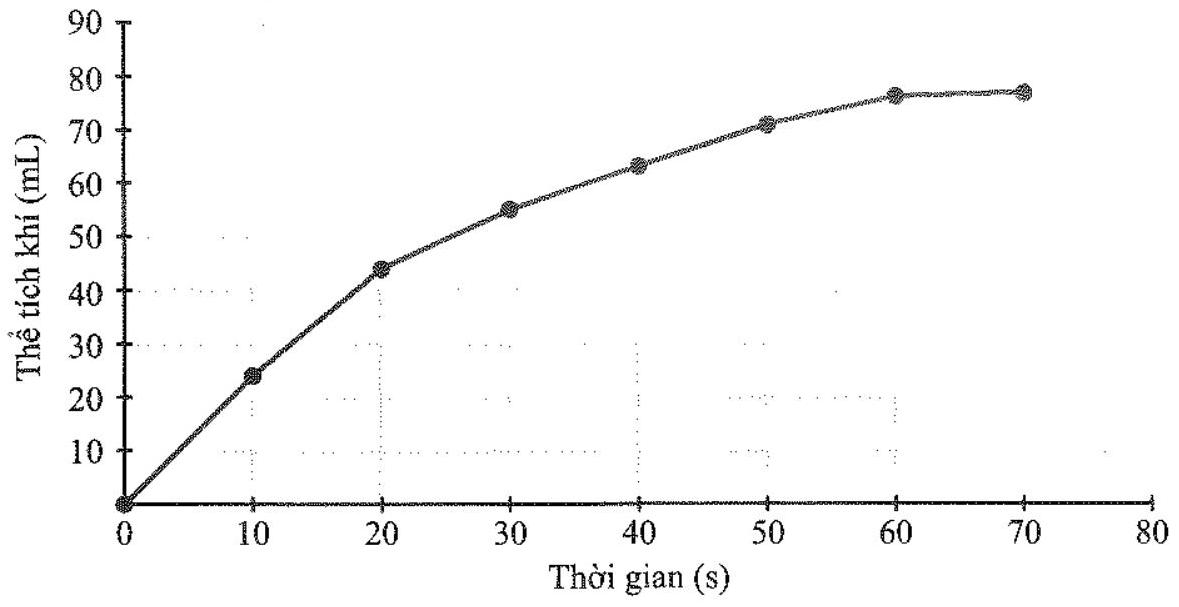
\includegraphics[max width=\textwidth, center]{2025_10_23_baf6b6057fd5ebd09626g-25}

Cần lặp lại thí nghiệm ba lần để giảm sai số trong quá trình thực nghiệm và tăng độ tin cậy của kết quả thu được.\\
c) Khoảng 70 giây phản ứng sẽ kết thúc vì khi đó khí thoát ra rất chậm và gần như không đổi.\\
d) Phản ứng nhanh nhất trong khoảng 10 giây đầu, sau đó chậm dần.\\
e) Nếu thí nghiệm được lặp lại với nồng độ HCl lớn hơn thì tốc độ phản ứng sẽ nhanh hơn.\\
g) Có thể thực hiện thí nghiệm bằng cách đặt bình phản ứng lên cân và theo dõi sự thay đổi khối lượng bình khi phản ứng diễn ra để tính khối lượng $\mathrm{H}_{2}$ thu được.\\
16.13. Tốc độ của phản ứng ở $40^{\circ} \mathrm{C}$ là: $v_{40}=v_{15} \times 3,5^{\frac{40-15}{10}}=4,6\left(\mathrm{M} \mathrm{s}^{-1}\right)$.\\
16.14. B, C, D.\\
16.15. B, D.\\
16.16. A, C.\\
16.17. B. 16.18. A.\\
16.19. $360 \times 24 \times 60 \times 60 \times 10^{-7}=3,11$ (giây).\\
16.20. 1. a) $\mathrm{H}_{2} \mathrm{O}_{2} \rightarrow \frac{1}{2} \mathrm{O}_{2}+\mathrm{H}_{2} \mathrm{O}$.\\
b) (1) oxygen; (2) đưa que đóm còn tàn đỏ sẽ thấy que đóm bùng cháy.\\
c) không còn thấy khí thoát ra.\\
d) lọc.

\section*{BÀI 17}
17.1. D.\\
17.2 a) A: fluorine, $\mathrm{F} ; \quad \mathrm{B}$ : bromine, $\mathrm{Br} ; \quad \mathrm{C}$ : iodine, $\mathrm{I} ; \quad \mathrm{D}$ : chlorine, Cl .\\
b) $\mathrm{F}_{2}, \mathrm{Br}_{2}, \mathrm{I}_{2}, \mathrm{Cl}_{2}$.\\
c) Học sinh tự trả lời dựa vào xu hướng biến đổi của mỗi tính chất vật lí của halogen.\\
17.3. A. 17.4. D. 17.5. A, B và D.\\
17.6. $\mathrm{a}-2,4,5,7 ; \mathrm{b}-1,3,4,6$.\\
17.7. $\mathrm{B}, \mathrm{C}$ và D .\\
17.8. $C$ và $D$. 17.9. $A$ 17.10. $D$. 17.11. $A, B, C$ và $D$.\\
17.12. Giải thích dựa vào thành phần và tính chất của các chất trong nước chlorine.\\
17.13. Làm giảm lượng chlorine dư trong nước sinh hoạt: chlorine phát tán vào không khí.\\
17.14. Học sinh chủ động tìm hiểu thông tin từ các nguồn học liệu khác nhau, có thể từ các nguồn học liệu số trên internet. Từ đó, học sinh xác định được sự đa dạng trong sử dụng chất khử khuẩn nước hồ bơi. Dưới đây là thông tin gợi ý.\\
Do khó bão quản trong vận chuyển và lưu trư, nước chlorine it được sử dụng để khư khuẩn nước hồ bơi. Hiện nay, trong thực tế, để cung cấp ion hypochlorite và hypochlorous acid có tính sát khuẩn cao, khử khuẩn cho hồ bơi, người ta có thể dùng nước Javel hoặc chlorine 70 (Ca(OCl)2 hay Ca(ClO) ${ }_{2}$, calcium hypochlorite dạng bột dễ bảo quản, lưu trũ và sử dụng. Chất này có hàm lượng ion hypochlorite lớn hơn so với nước Javel khoảng 70\%). Do ion hypochlorite và hypochlorous acid dễ bị phân huỷ khi tiếp xúc trục tiếp với ánh sáng mặt trời nên việc khử khuẩn hồ bơi thường được thực hiện vào ban đêm.\\
Ngoài ra, người ta còn sử dụng hoá chất TCCA 90 dạng viên chưa hợp chất trichloroisocyanuric acid ( $\mathrm{C}_{3} \mathrm{Cl}_{3} \mathrm{~N}_{3} \mathrm{O}_{3}$ ). Hợp chất này khi tan trong nước tạo thành hypochlorous acid và cyanuric acid. Trong đó, cyanuric acid có tác dụng ổn định tính khư khuẩn của hypochlorous acid dưới tác dụng của ánh sáng mặt trời.\\
17.15. B. Theo đặc điểm của phản ứng: Khi 1 mol hỗn hợp muối ( $\mathrm{NaBr}, \mathrm{KBr}$ ) chuyển thành 1 mol hỗn hợp muối $(\mathrm{NaCl}, \mathrm{KCl})$ thì khối lượng giảm:

$$
80-35,5=44,5(\mathrm{gam})
$$

Theo đề bài: Khối lượng muối trong thí nghiệm đã giảm 4,45 gam.\\
Vậy $\mathrm{n}_{\text {muối }}=\mathrm{n}_{\mathrm{Cl}(\text { phản ứng })}=4,45: 44,5=0,10(\mathrm{~mol})$.\\
Nên $\mathrm{n}_{\mathrm{Cl}_{2}}=0,10: 2=0,05(\mathrm{~mol})$.\\
17.16, a) A.\\
b) Lượng acid thương phẩm được tạo ra cùng 200 gam xút:

$$
\frac{\frac{200}{40} \times 36,5 \times 0,6 \times 0,8}{0,32 \times 1,153}=237,4(\mathrm{~mL}) .
$$

Vậy với 200 tấn $=200 \times 10^{6}$ gam xút thì lượng acid thương phẩm được tạo thành tương ứng là: $237,4 \mathrm{~mL} \times 10^{6}=237,4 \mathrm{~m}^{3}$.\\
17.17. D. Có thể nhận thấy potassium không thay đổi số oxi hoá ( +1 trong các hợp chất). Số oxi hoá của iodine trong đơn chất và potassium iodide lần lượt là 0 , -1 và giữa chúng không có số oxi hoá trung gian. Như vậy, trong phản ứng này không có sự thay đổi số oxi hoá của các nguyên tố, do đó không phải là phản ứng oxi hoá - khử. Thực tế, phản ứng này là sự kết hợp giữa ion $\mathrm{I}^{-}$và phân tử $I_{2}$ tạo ion $I_{3}^{-}$bằng một liên kết cho - nhận.\\
Trong thực tế, phản ứng này giúp chuyển iodine ( $\mathrm{I}_{2}$, ít tan trong nước) thành ion triodine ( $\mathrm{I}_{3}^{-}$, tan tốt trong nước) phân tán dễ dàng vào dung dịch. Dung dịch này có tính sát khuẩn.\\
17.18. A.\\
17.19. a) Xét các phản ứng:


\begin{equation*}
\mathrm{X}_{2}(g)+\mathrm{H}_{2}(g) \rightarrow 2 \mathrm{HX}(g) \quad \Delta_{\mathrm{r}} \mathrm{H}_{298}^{0} \tag{}
\end{equation*}


Biến thiên enthalpy chuẩn được tính theo công thức:

$$
\Delta_{\mathrm{r}} \mathrm{H}_{298}^{0}(*)=\left(1 \times \mathrm{E}_{(\mathrm{X}-\mathrm{X})}+1 \times \mathrm{E}_{(\mathrm{H}-\mathrm{H})}\right)-2 \times \mathrm{E}_{(\mathrm{H}-\mathrm{X})}
$$

Cu ̣ thể, với phản ứng: $\mathrm{Cl}_{2}(g)+\mathrm{H}_{2}(g) \rightarrow 2 \mathrm{HCl}(g)$

$$
\Delta_{\mathrm{r}} \mathrm{H}_{298}^{0}=(1 \times 243+1 \times 436)-2 \times 431=-183(\mathrm{~kJ}) .
$$

Tương tự: $\mathrm{Br}_{2}(g)+\mathrm{H}_{2}(g) \rightarrow 2 \mathrm{HBr}(g)$

$$
\Delta_{\mathrm{r}} \mathrm{H}_{298}^{0}=-99 \mathrm{~kJ}
$$

$$
\mathrm{I}_{2}(g)+\mathrm{H}_{2}(g) \rightarrow 2 \mathrm{HI}(g)
$$

$$
\Delta_{\mathrm{r}} \mathrm{H}_{298}^{0}=-7 \mathrm{~kJ} .
$$

b) Nhiệt lượng toả ra trong phản ứng của $\mathrm{Cl}_{2}>\mathrm{Br}_{2}>\mathrm{I}_{2}$. Phản ứng có giá trị biến thiên enthalpy chuẩn càng âm thì toả nhiệt càng nhiều.\\
17.20. a) Liên kết bền nhất là H-F. Năng lượng liên kết càng lớn thì liên kết càng bền.\\
b) -535 và -486 kJ .\\
c) Phản ứng (1) toả ra nhiều nhiệt hơn. Phản ứng có giá trị biến thiên enthalpy chuẩn âm hơn thì sẽ toả nhiệt nhiều hơn.\\
17.21. a) Với phản ứng:

$$
2 \mathrm{Br}^{-}(a q)+\mathrm{Cl}_{2}(a q) \rightarrow 2 \mathrm{Cl}^{-}(a q)+\mathrm{Br}_{2}(a q)
$$

Dựa vào enthalpy tạo thành chuẩn của các chất, biến thiên enthalpy chuẩn của phản ứng được tính như sau:

$$
\begin{aligned}
\Delta_{\mathrm{r}} \mathrm{H}_{298}^{0}=2 \times \Delta_{\mathrm{f}} \mathrm{H}_{298}^{0}\left(\mathrm{Cl}^{-}(a q)\right)+\Delta_{\mathrm{f}} \mathrm{H}_{298}^{0}\left(\mathrm{Br}_{2}(a q)\right)-2 \times \Delta_{\mathrm{f}} \mathrm{H}_{298}^{0}\left(\mathrm{Br}^{-}(a q)\right) & -\Delta_{\mathrm{f}} \mathrm{H}_{298}^{0}\left(\mathrm{Cl}_{2}(a q)\right) \\
= & 2 \times(-167,16)+1 \times(-2,16)-2 \times(-121,55)-1 \times(-17,30) \\
= & -76,08(\mathrm{~kJ})
\end{aligned}
$$

b) Đây là phản ứng toả nhiệt nên thuận lợi về mặt năng lượng. Thực tế, phản ứng trên diễn ra dễ dàng.\\
17.22. a) Sau khi đo, sẽ tính được tỉ lệ $\mathrm{h} 1: \mathrm{h} 2=\mathrm{k}$ ( k là một số cụ thể).\\
b) Khoảng k lần.\\
c) Thay k vào các biểu thức sau để tính \% số nguyên tử mỗi đồng vị:

$$
\%{ }^{35} \mathrm{Cl}=\frac{\mathrm{k}}{\mathrm{k}+1} \times 100 \% ; \%{ }^{37} \mathrm{Cl}=\frac{1}{\mathrm{k}+1} \times 100 \%
$$

d) Nguyên tử khối trung bình của chlorine là:

$$
\overline{\mathrm{A}}=\frac{\%^{35} \mathrm{Cl} \times 35+\%^{37} \mathrm{Cl} \times 37}{\%^{35} \mathrm{Cl}+\%^{37} \mathrm{Cl}} \text { hay } \frac{\mathrm{k} \times 35+37}{\mathrm{k}+1}
$$

Tuỳ theo mức độ sai số khi đo h1 và h2 mà học sinh sẽ tính được giá trị k không nhất thiết trùng nhau. Vì vậy, giá trị nguyên tử khối trung bình mỗi học sinh tính được sẽ có sai biệt, nhưng không đáng kể.\\
Giá trị nguyên tử khối trung bình xác định được có thể dao động từ 35,45 đến 35,49 .

\section*{BAI 18}
18.1. $\mathrm{A}, \mathrm{B}, \mathrm{C}$ và D .\\
18.2.C.\\
18.3. $\mathrm{A}, \mathrm{D}$ và E .\\
18.4. $A$ và $C$.\\
18.5. D và E .\\
18.6. $\mathrm{A}, \mathrm{B}, \mathrm{C}, \mathrm{G}$ và H .\\
18.7.a-1,2,3; $\quad b-5,7 ; \quad c-1 ; \quad d-4,6,7$.\\
18.8. C và D .\\
18.9. Giải thích trên cơ sở tìm hiểu từ nội dung đã học về liên kết hydrogen: "Liên kết hydrogen là một loại liên kết yếu được hình thành giữa nguyên tử H (đã liên kết với một nguyên tử có độ âm điện lớn) với một nguyên tử khác (có độ âm điện lớn) còn cặp electron riêng. Các nguyên tử có độ âm điện lớn thường gặp trong liên kết hydrogen là $\mathrm{N}, \mathrm{O}, \mathrm{F}$."\\
18.10. Đề xuất trên cơ sở cách phân biệt các ion halide trong dung dịch.\\
18.11. a) $16 \mathrm{HCl}(a q)+2 \mathrm{KMnO}_{4}(s) \rightarrow 2 \mathrm{KCl}(a q)+2 \mathrm{MnCl}_{2}(a q)+5 \mathrm{Cl}_{2}(a q) +8 \mathrm{H}_{2} \mathrm{O}(l)$\\
b) $\mathrm{MnO}_{2}(s)+4 \mathrm{HCl}(a q) \rightarrow \mathrm{MnCl}_{2}(a q)+\mathrm{Cl}_{2}(g)+2 \mathrm{H}_{2} \mathrm{O}(l)$\\
c) $3 \mathrm{Cl}_{2}(g)+6 \mathrm{NaOH}(a q) \rightarrow 5 \mathrm{NaCl}(a q)+\mathrm{NaClO}_{3}(a q)+3 \mathrm{H}_{2} \mathrm{O}(l)$\\
d) $2 \mathrm{NaBr}(a q)+3 \mathrm{H}_{2} \mathrm{SO}_{4}(l) \rightarrow 2 \mathrm{NaHSO}_{4}(s)+\mathrm{Br}_{2}(g)+\mathrm{SO}_{2}(g)+2 \mathrm{H}_{2} \mathrm{O}(g)$\\
e) $8 \mathrm{HI}(g)+\mathrm{H}_{2} \mathrm{SO}_{4}(l) \rightarrow 4 \mathrm{I}_{2}(g)+\mathrm{H}_{2} \mathrm{~S}(g)+4 \mathrm{H}_{2} \mathrm{O}(l)$\\
18.12. a) Hydrogen iodide\\
b) Sodium chloride\\
c) KI\\
d) Sodium hypochlorite.\\
18.13. a)

\begin{center}
\begin{tabular}{|l|l|l|l|l|}
\hline
Timh chất & \multicolumn{4}{|c|}{Chiều tăng tính chất} \\
\hline
Độ âm điện nguyên tố X & I & Br & Cl & F \\
\hline
Tính oxi hoá của đơn chất $\mathrm{X}_{2}$ & $\mathrm{I}_{2}$ & $\mathrm{Br}_{2}$ & $\mathrm{Cl}_{2}$ & $\mathrm{F}_{2}$ \\
\hline
Tính khử của ion $\mathrm{X}^{-}$ & $\mathrm{F}^{-}$ & $\mathrm{Cl}^{-}$ & $\mathrm{Br}^{-}$ & $\mathrm{I}^{-}$ \\
\hline
Tính acid của hợp chất HX & HF & HCl & HBr & HI \\
\hline
\end{tabular}
\end{center}

b) Phản ứng với sulfuric acid đặc trong cùng điều kiện:\\
$\mathrm{NaF}(s)+\mathrm{H}_{2} \mathrm{SO}_{4}(l) \rightarrow \mathrm{NaHSO}_{4}(s)+\mathrm{HF}(g)$\\
$\mathrm{NaCl}(s)+\mathrm{H}_{2} \mathrm{SO}_{4}(l) \rightarrow \mathrm{NaHSO}_{4}(s)+\mathrm{HCl}(g)$\\
$2 \mathrm{NaBr}(s)+3 \mathrm{H}_{2} \mathrm{SO}_{4}(l) \rightarrow 2 \mathrm{NaHSO}_{4}(s)+\mathrm{SO}_{2}(g)+\mathrm{Br}_{2}(g)+2 \mathrm{H}_{2} \mathrm{O}(g)$\\
$8 \mathrm{NaI}(s)+9 \mathrm{H}_{2} \mathrm{SO}_{4}(l) \rightarrow 8 \mathrm{NaHSO}_{4}(s)+\mathrm{H}_{2} \mathrm{~S}(g)+4 \mathrm{I}_{2}(g)+4 \mathrm{H}_{2} \mathrm{O}(g)$\\
Dễ nhận thấy $\mathrm{F}^{-}$và $\mathrm{Cl}^{-}$không thể hiện tính khử, $\mathrm{Br}^{-}$khử lưu huỳnh có số oxi hoá +6 về số oxi hoá +4 ; $\mathrm{I}^{-}$có thể khử lưu huỳnh có số oxi hoá +6 về số oxi hoá thấp hơn, -2 . Vậy tính khử $\mathrm{I}^{-}>\mathrm{Br}^{-}>\mathrm{Cl}^{-}, \mathrm{F}^{-}$.\\
Mặt khác, $\mathrm{Cl}^{-}$trong HCl đặc có thể khử $\mathrm{MnO}_{2}$ theo phản ứng sau:

$$
4 \mathrm{HCl}(a q)+\mathrm{MnO}_{2}(s) \rightarrow \mathrm{MnCl}_{2}(a q)+\mathrm{Cl}_{2}(g)+2 \mathrm{H}_{2} \mathrm{O}(l)
$$

Phản ứng này dùng điều chế chlorine trong phòng thí nghiêm, trong khi đó $\mathrm{F}^{-}$trong điều kiện tương tự thì không xảy ra phản ứng. Ngoài ra, $\mathrm{F}^{-}$hầu như không thể bị oxi hoá bởi các hoá chất khác trong điều kiện thông thường.\\
Vậy tính khử $\mathrm{Cl}^{-}>\mathrm{F}^{-}$.\\
c) Nguyên nhân chủ yếu làm tăng độ mạnh của các acid theo dãy trên là do sự giảm độ bền liên kết theo thứ tự: $\mathrm{H}-\mathrm{F}>\mathrm{H}-\mathrm{Cl}>\mathrm{H}-\mathrm{Br}>\mathrm{H}-\mathrm{I}$.\\
18.14. a) $\mathrm{HCl}+\mathrm{HC} \equiv \mathrm{CH} \rightarrow \mathrm{H}_{2} \mathrm{C}=\mathrm{CHCl} ; \quad \mathrm{HCl}+\mathrm{NH}_{3} \rightarrow \mathrm{NH}_{4} \mathrm{Cl}$.\\
b) Sản xuất nhựa PVC và sản xuất phân đạm.\\
18.15. a) $\mathrm{FeO}(s)+2 \mathrm{HCl}(a q) \rightarrow \mathrm{FeCl}_{2}(a q)+\mathrm{H}_{2} \mathrm{O}(l)$

$$
\begin{aligned}
& \mathrm{Fe}_{2} \mathrm{O}_{3}(s)+6 \mathrm{HCl}(a q) \rightarrow 2 \mathrm{FeCl}_{3}(a q)+3 \mathrm{H}_{2} \mathrm{O}(l) \\
& \mathrm{Fe}(s)+2 \mathrm{HCl}(a q) \rightarrow \mathrm{FeCl}_{2}(a q)+\mathrm{H}_{2}(g) \\
& \mathrm{Fe}(s)+2 \mathrm{FeCl}_{3}(a q) \rightarrow 3 \mathrm{FeCl}_{2}(a q)
\end{aligned}
$$

b) Phản ứng diễn ra ở nhiệt độ cao, thu khí hydrogen chloride. Khí này cần được hoà tan vào nước để thu lại hydrochloric acid, dung dịch này được tái sử dụng.\\
18.16. a) Dựa vào định nghĩa enthalpy tạo thành chuẩn của chất, học sinh biết được giá trị cần điền.\\
b) -350 kJ .\\
c) Phản ứng oxi hoá acid bởi oxygen thuận lợi về năng lượng. Khi đung dịch hydroiodic acid tiếp xúc với không khí, dung dịch bị biến đổi (thành phần, màu sắc) theo phản ứng:

$$
4 \mathrm{HI}(a q)+\mathrm{O}_{2}(g) \rightarrow 2 \mathrm{H}_{2} \mathrm{O}(l)+2 \mathrm{I}_{2}(s)
$$

d) Giảm sự tiếp xúc của dung dịch với oxygen có trong không khí.\\
18.17. a) 118 kJ và 63 kJ .\\
b) Thu nhiệt từ môi trường.


\end{document}